\documentclass[11pt,a4paper]{article}
\usepackage[T1]{fontenc}
\usepackage[utf8]{inputenc}
\usepackage{lmodern}
\usepackage[a4paper,margin=2.5cm]{geometry}
\usepackage{amsmath,amssymb,booktabs,graphicx,array,multirow,xcolor}
\usepackage[font=small,labelfont=bf]{caption}
\usepackage{subcaption}
\usepackage{rotating}
\usepackage{tikz}
\usetikzlibrary{positioning,arrows.meta,calc,fit}
\usepackage[hidelinks]{hyperref}
\usepackage{enumitem}
\usepackage{microtype}
\setlength{\textfloatsep}{12pt plus 2pt minus 2pt}\setlength{\floatsep}{10pt plus 2pt minus 2pt}\setlength{\intextsep}{10pt plus 2pt minus 2pt}
\renewcommand{\topfraction}{0.9}\renewcommand{\bottomfraction}{0.8}\renewcommand{\textfraction}{0.08}\renewcommand{\floatpagefraction}{0.8}
\usepackage[section]{placeins}
\setlist{itemsep=1pt,topsep=3pt}
\graphicspath{{figures/}}
\newcommand{\coderepo}{https://github.com/sid200510/Critical-Node-Identification}

\title{\textbf{Ranking and Identifying Critical Agents in\\ Simulated Aerial Swarms with a Graph Neural Network}}
\author{K.\ Sai Siddhartha Bajrang \quad (AE22B002)\\[3pt]
\small AE5510 Security of Safety-Critical Systems --- Final Project Report (Problem 2)\\
\small Guide: Devaprakash Muniraj, Department of Aerospace Engineering}
\date{20 November 2026}

\begin{document}
\maketitle

\begin{abstract}
\noindent
This project looks at how to identify the important agents in a simulated aerial swarm. An agent may be important because of its position in the formation or because it connects different parts of the communication network. I use a graph neural network to give each alive agent a criticality score at every timestep. The scores are used both to rank the agents and to decide which ones are critical. At each step, agents within the 55-unit sensing range are connected to form a graph. The model uses edge-aware GIN (GINE) layers, feature attention and a swarm-level readout. It is trained using a differentiable ranking loss along with a weighted classification loss.

I tested the model on swarm conditions that were not used for training, including different swarm sizes, attrition levels and obstacle densities. The split contains 17 training, 41 validation and 42 test swarms. On the test set, the model achieves a per-timestep Spearman correlation of about 0.82 and an AUPRC of 0.87, compared with a random-score AUPRC of 0.39. The F1 score is 0.78 and recall is 0.81. When the predictions are averaged over a mission, the ranking correlation increases to 0.86 and AUPRC to 0.93. The results are also encouraging for larger unseen swarms of 52--75 agents, where the ranking correlation is around 0.85--0.86. Performance is weaker at the start of a mission and improves later. I also found that adding the classification loss helps detection without reducing ranking performance, while the extra within-swarm relative features make little difference at $d=12$. Position noise is a more serious issue than velocity noise because it can change the graph connections; at 20\,\% position noise, the ranking correlation falls to 0.71.

\end{abstract}

\noindent\textbf{Code repository:} \url{\coderepo}

\section{Introduction}
\FloatBarrier
\subsection{Problem}
The data consists of 100 simulated swarm missions, referred to as cases. The cases have different numbers of agents
($N\in\{18,24,30,37,45,52,60,68,75\}$), levels of attrition (none, light, medium or heavy), obstacle densities and clutter indices.
Each row describes one agent at one timestep. It includes its position relative to the swarm centroid, velocity, heading,
flight-path angle, acceleration, neighbourhood information and four graph-centrality measures. There are two targets:
a continuous \texttt{criticality\_score} between 0 and 1, and a binary \texttt{is\_critical} label. Around 39\,\% of the
agent-timestep rows are labelled critical. My aim is to use these inputs to rank the agents by criticality and identify
critical agents, including in swarms with operating conditions not seen during training.

\FloatBarrier
\subsection{Motivation}
One reason to use a swarm is that the system should not depend too much on any one agent. However, some agents can still
be more important than others. For example, an agent might connect two groups or help keep the formation together.
Knowing which agents matter most can help an operator decide where to provide protection or backup. It can also help
assess a hostile swarm by identifying high-priority agents \cite{teng2024drones}. A ranked list is useful here because
there may not be enough resources to act on every agent, and a simple critical/non-critical label does not show the
relative importance of agents.

In Review~2, I found that the four standard centrality measures and a community-aware betweenness measure did not
separate the two classes well for this dataset. Models based on manually calculated trajectory statistics also gave
only moderate performance (test F1 between 0.72 and 0.84). This suggested that an agent's importance could depend on
the rest of the swarm, rather than only on its individual trajectory. That is the main reason for trying a graph neural network.

\FloatBarrier
\subsection{Questions addressed}
\begin{enumerate}[label=\arabic*.]
\item How well can one model both rank agents and identify the critical ones on unseen swarm sizes and conditions?
\item Which design choices matter: latent size, within-swarm relative features, the classification term (Section~\ref{sec:design})?
\item How does performance depend on mission time, swarm size, attrition and obstacle density, and which inputs does the model rely on?
\item How robust are the predictions to noisy positions and velocities?
\end{enumerate}

\section{Literature review}\label{sec:lit}

\paragraph{Critical nodes.} A critical node is usually understood as one whose removal causes a large drop in some measure
of network connectivity. Finding the best set of nodes to remove is generally NP-hard. Lalou et al.\ \cite{lalou2018cndp}
review exact, approximate and heuristic approaches, including methods based on degree, closeness, betweenness and
eigenvector centrality. In a drone-swarm setting, Teng et al.\ \cite{teng2024drones} construct a communication graph
using the drones' 3-D positions and communication range. They then use a community-aware centrality measure and check
how removing selected drones affects the network. These methods are useful starting points, but they mostly describe
the network at one instant. They also do not directly use how the agents are moving. In Review~2, the four centrality
features by themselves did not give a good separation of critical and non-critical agents.

\paragraph{Learning to rank nodes with GNNs.} Fan et al.\ \cite{fan2019drbc} propose DrBC, which uses a GNN to learn
which nodes have high betweenness centrality. They train on small synthetic graphs with a pairwise ranking loss and
then test on much larger graphs. This is relevant to my project because I also want a model trained on some swarm
sizes to work on sizes it has not seen before. The main difference is that DrBC predicts a static centrality,
whereas my target is the simulator's criticality score for moving agents in a graph that changes over time.

\paragraph{Graph layers.} The graph isomorphism network (GIN) \cite{xu2019gin} adds the feature vectors of neighbouring
nodes and then passes the result through an MLP,
$h_i'=\mathrm{MLP}\big((1+\epsilon)h_i+\sum_j h_j\big)$. The sum is useful because it retains information
about how many neighbours a node has, unlike a simple mean. GIN also has strong distinguishing power related to
the Weisfeiler--Lehman test. GINE \cite{hu2020gine} extends this by including edge features in the messages,
$\mathrm{ReLU}(h_j+W_e e_{ij})$. I use this version so that the distance between two agents can affect the message passed between them.

\paragraph{Optimising a ranking.} There is a difficulty in directly training for Spearman correlation or other rank
metrics: the ranks do not change smoothly as the predicted scores change, so ordinary backpropagation cannot optimise
them directly. Qin et al.\ \cite{qin2010} suggest approximating rank positions with sigmoids of pairwise score
differences. This gives a smooth approximation that can be used in a loss function. I follow this idea for the ranking loss.

\paragraph{Gap.} Most of the node-ranking work I looked at either learns an existing centrality score or uses a
hand-designed score for a graph snapshot. For this project, I wanted to see whether one model could learn both the
continuous ranking and the binary label from a changing swarm graph, and whether it would still work when swarm size,
attrition or obstacle density was different from the training cases. The cited work does not directly evaluate this
combination of tasks and held-out conditions.

\section{Methodology}\label{sec:method}

\subsection{Graphs and features}
I use every third recorded timestep to keep the dataset manageable. At time $t$, the agents that are still alive,
$A(t)$, form a graph. Two agents are connected when their distance is at most 55 units, which is the sensing range:
$(i,j)$ is an edge if $\lVert p_i(t)-p_j(t)\rVert\le55$. The edge feature is the normalised distance
$e_{ij}=d_{ij}/55$. Each node has the 34 features listed in Table~\ref{tab:features}. I encode angles with sine
and cosine so that the change from $\pi$ to $-\pi$ does not appear as a large jump. If an agent has no neighbour
within range, its missing neighbour-distance value is set to 55. The 11 relative features describe an agent
compared with the other alive agents at that timestep, using within-swarm $z$-scores:

\begin{equation}
x^{\mathrm{rel}}_{i,f}(t)=\frac{x_{i,f}(t)-\mu_f(t)}{\sigma_f(t)},\qquad \mu_f(t),\sigma_f(t)\ \text{over } A(t),
\end{equation}
These relative values show whether an agent is unusually fast, central or well-connected compared with the rest of
its swarm. They may also reduce differences caused by changes in swarm size or operating conditions. Missing values
are filled with the training median, and the features are standardised using statistics computed only on the training swarms.

\begin{table}[!htbp]\centering\small
\caption{The 34 inputs per agent and timestep.}\label{tab:features}
\begin{tabular}{@{}lcp{10.9cm}@{}}\toprule
Group & No. & Features\\\midrule
Dynamics & 11 & $v_x,v_y,v_z$, speed, acceleration, heading rate, angular coverage, $\sin/\cos$ heading, $\sin/\cos$ flight-path angle\\
Position & 4 & position relative to the swarm centroid $(x,y,z)$, distance to centroid\\
Neighbourhood & 4 & number of neighbours, mean and minimum neighbour distance, distance-weighted density\\
Centrality & 4 & degree, closeness, betweenness, eigenvector centrality (from the simulator)\\
Relative & 11 & within-swarm $z$-scores of the 4 neighbourhood and 4 centrality features, distance to centroid, angular coverage, speed\\\bottomrule
\end{tabular}
\end{table}

\subsection{Out-of-distribution split}
I split the data by complete missions rather than by individual rows. Otherwise, timesteps from almost the same
mission could appear in both training and testing, making the results too optimistic. I hold out any case with
$N\in\{52,68,75\}$, light or heavy attrition, or obstacle density below 0.07. This leaves 17 cases for training.
The other 83 cases are randomly divided, with seed 42, into 41 validation and 42 test cases. Every validation and
test mission therefore has at least one condition that was not present in training. I select the model using only
validation results and use the test set for the final evaluation.

\subsection{Baselines}
For reference, I include the baselines from Review~2. These models predict whether an agent is critical using
statistics of its full trajectory. For each of four signals ($x,y,z$ relative to the centroid and distance to the
target), I calculated seven values: mean, standard deviation, minimum, maximum, median, last minus first and a
linear slope. This produces a 28-dimensional feature vector per agent. I trained logistic regression with median
imputation, standardisation and balanced class weights, and gradient boosting with 200 trees, depth 3 and learning
rate 0.05. The earlier GNN baseline used three GIN layers, mean pooling over time and only a classification loss.

An important difference is that Review~2 used an easier split of 31 training, 34 validation and 35 test missions.
It held out sizes 52 and 68, high or heavy attrition, or obstacle density below 0.07. Because that split is not
the one used here, the earlier scores are useful context rather than a direct comparison. The baseline pipeline
and results are shown in Figure~\ref{fig:baselines}.

\begin{figure}[!t]\centering
\begin{subfigure}{\textwidth}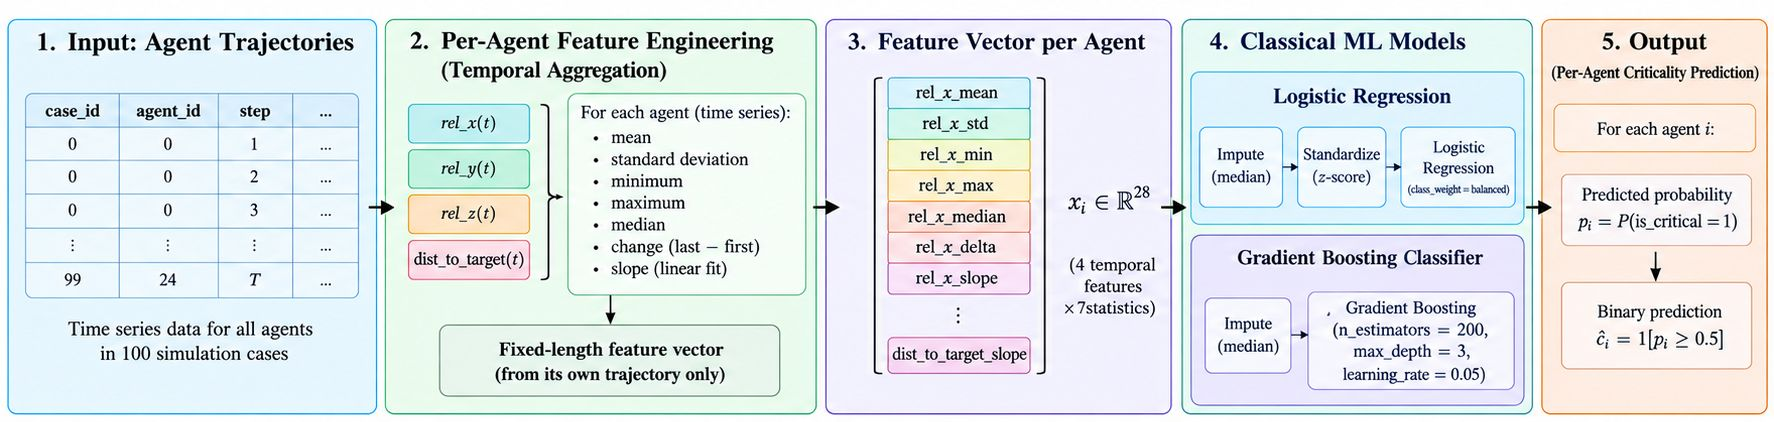
\includegraphics[width=\linewidth]{review2_baseline_pipeline.png}\caption{Feature-engineering baseline. Each agent's trajectory is summarised by seven statistics of four time series, and the resulting 28-dimensional vector is classified with logistic regression or gradient boosting.}\end{subfigure}\\[6pt]
\begin{subfigure}{\textwidth}\centering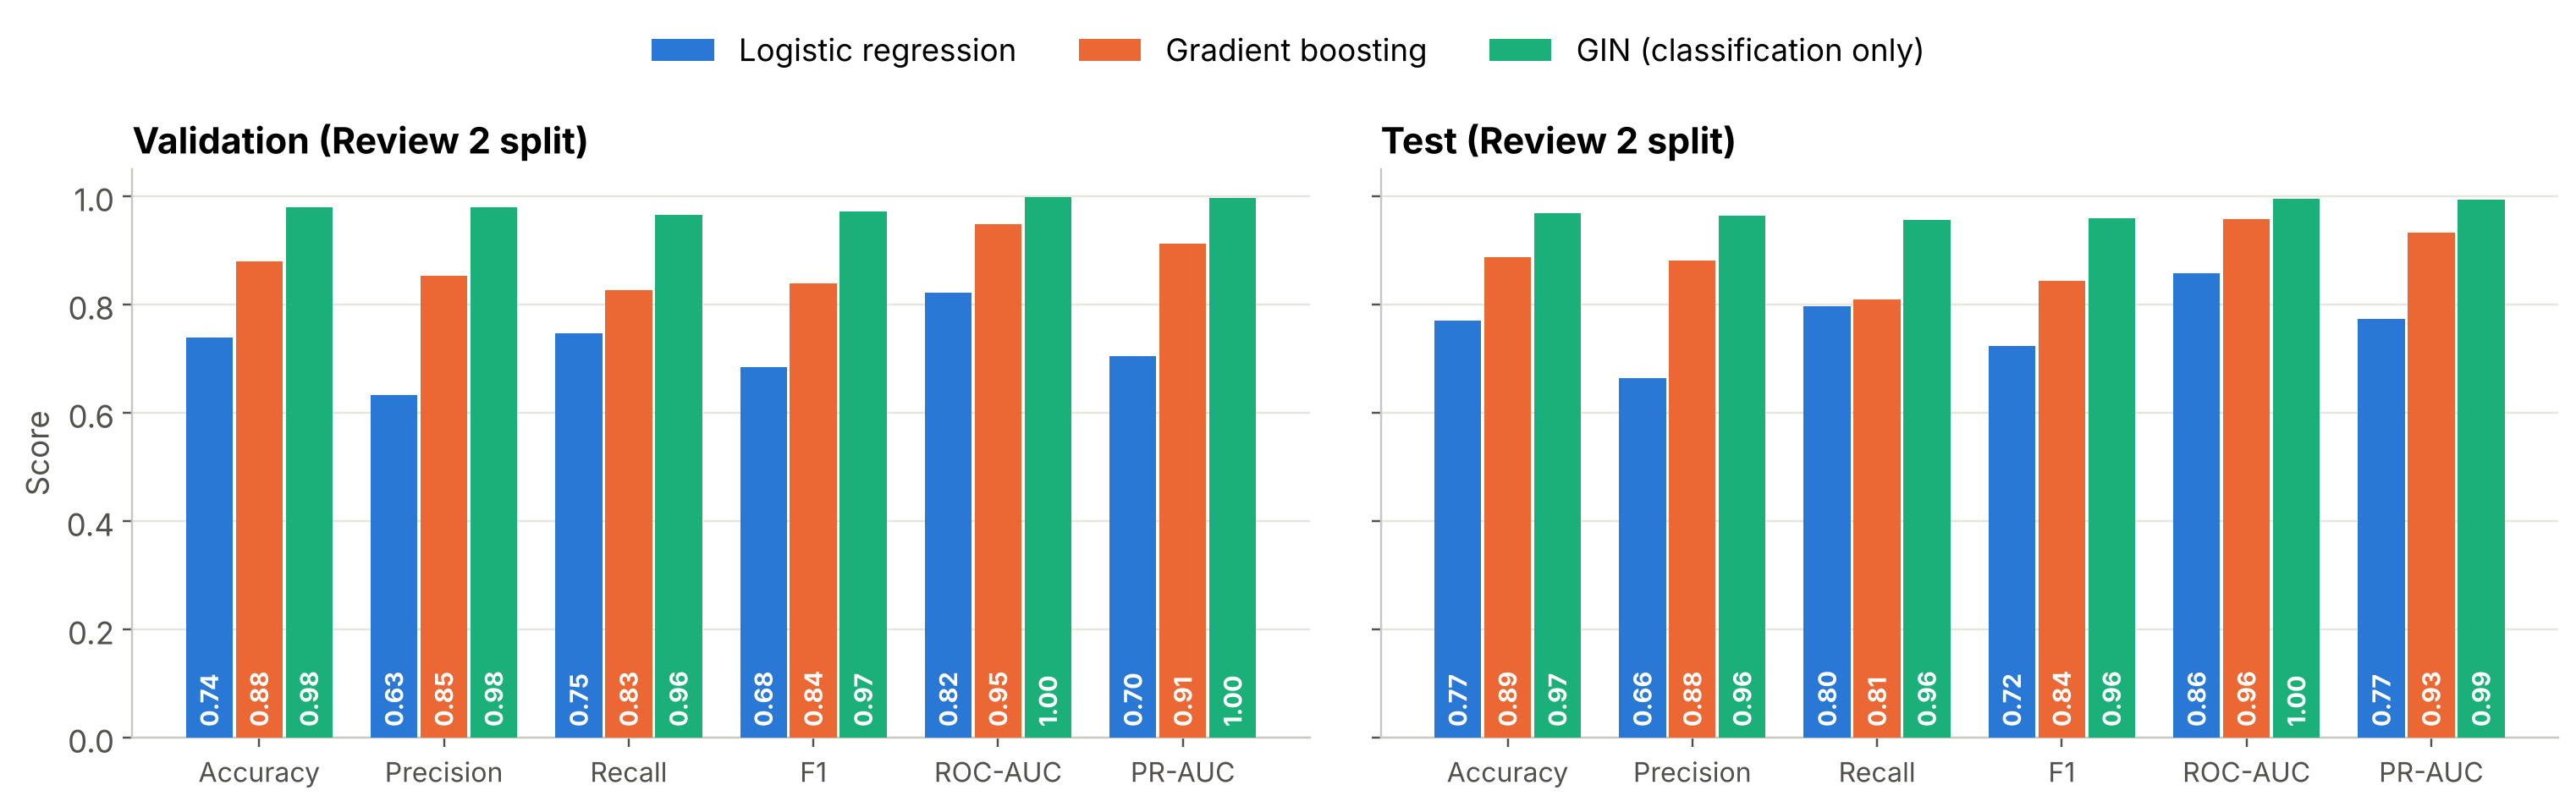
\includegraphics[width=0.92\linewidth]{review2_baseline_results.png}\caption{Validation and test scores of the Review~2 models for the agent-level classification of \texttt{is\_critical}, evaluated on the Review~2 split.}\end{subfigure}
\caption{Baseline models from Review~2. Gradient boosting is clearly better than logistic regression (test F1 0.84 vs 0.72), which suggests a non-linear relation between trajectory statistics and criticality. The near-perfect GIN scores were obtained on an easier split and for classification only, so they are not directly comparable with the results of this report.}\label{fig:baselines}
\end{figure}


\FloatBarrier
\subsection{Model}
The model architecture is shown in Figure~\ref{fig:arch}. I chose to predict a score separately at each timestep
instead of combining an agent's whole trajectory. This means the model can update its ranking as the swarm changes,
without needing the future part of the mission.

\begin{sidewaysfigure}\centering
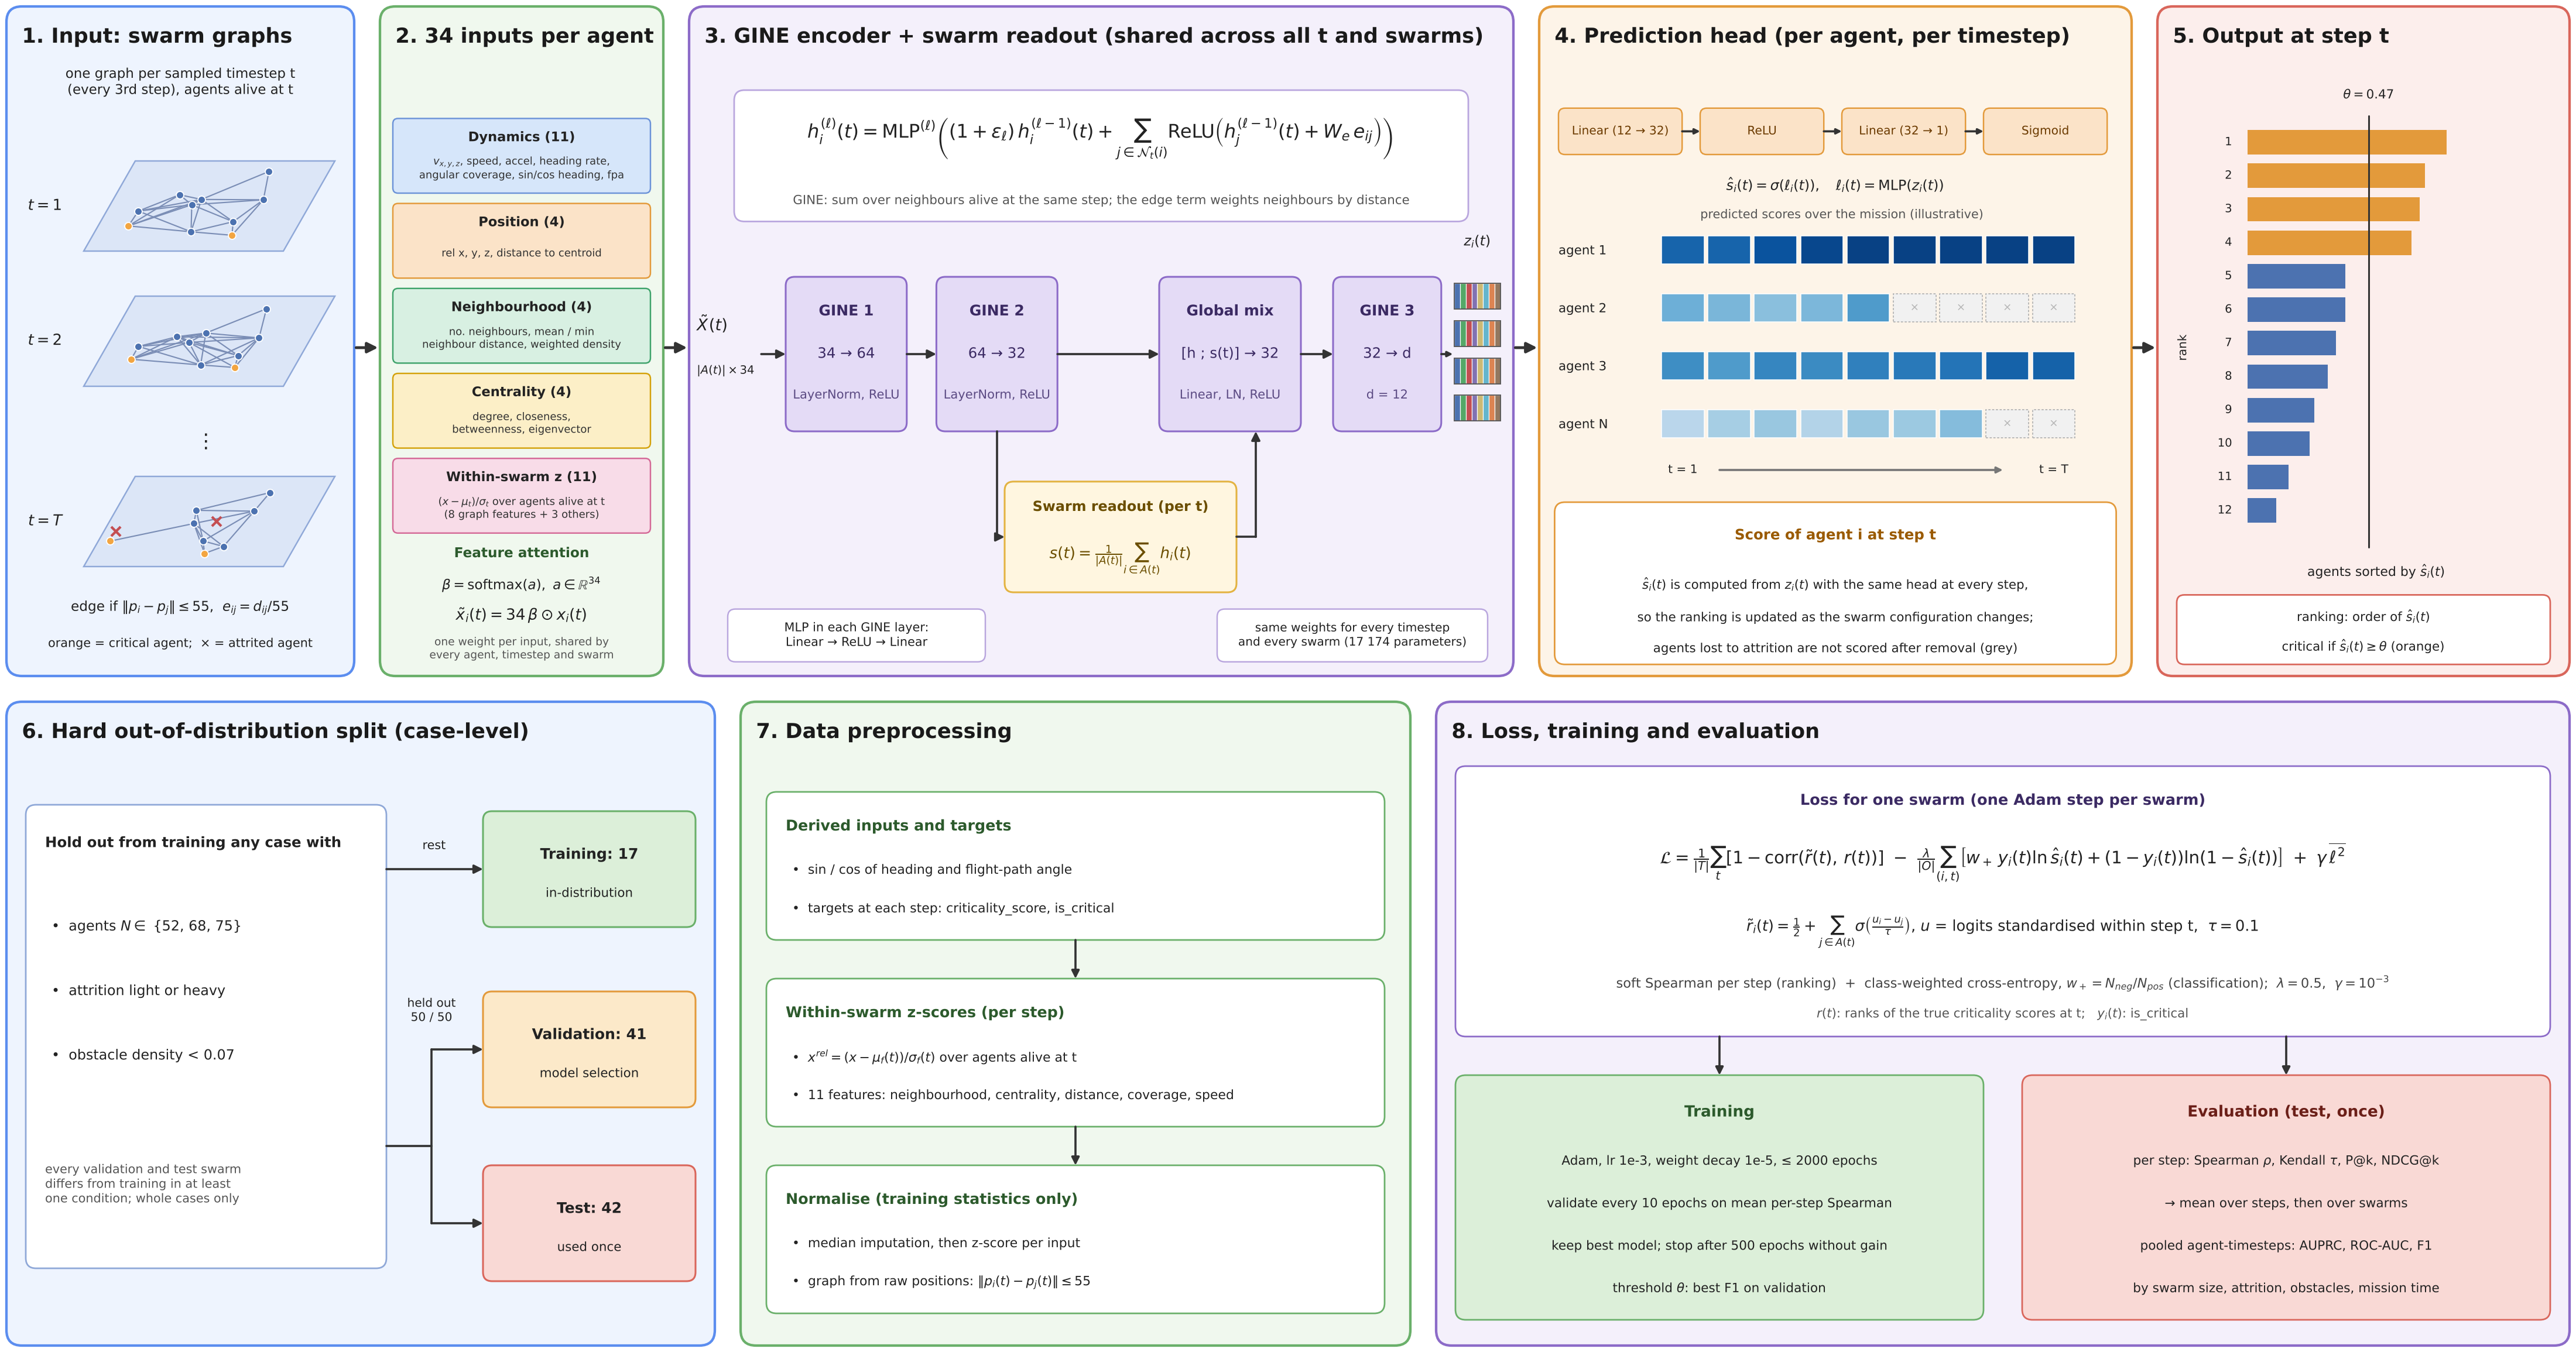
\includegraphics[width=\textwidth]{architecture_per_timestep.png}
\caption{Architecture of the proposed model. Panels 1--5 show the forward pass: a proximity graph is built at every sampled timestep, the 34 inputs are rescaled by a learned feature attention, three GINE layers with a swarm readout produce a latent state $z_i(t)$ for each agent, and a shared MLP head maps it to a criticality score $\hat s_i(t)$, from which the ranking and the critical agents at that step are obtained. Panels 6--8 summarise the data split, the preprocessing and the training objective. Because all weights are shared across agents, timesteps and swarms, the same model can be applied to swarms of any size.}
\label{fig:arch}
\end{sidewaysfigure}


\paragraph{Feature attention.} I use one trainable weight for each input feature. The weights are calculated as
$\beta=\mathrm{softmax}(a)$, and the inputs become $\tilde x=F\,\beta\odot x$, where $F=34$.
The factor $F$ keeps the input unchanged when all features have equal weight. The same weights are used for all
agents and timesteps. Looking at them later gives an indication of which inputs the model uses more strongly
(Section~\ref{sec:features}).

\paragraph{GINE layers.} The graph is processed using three edge-aware GIN layers \cite{xu2019gin,hu2020gine}.
The update for a node is

\begin{equation}
h_i'=\mathrm{MLP}\Big((1+\epsilon)\,h_i+\sum_{j\in\mathcal{N}_t(i)}\mathrm{ReLU}\big(h_j+W_e\,e_{ij}\big)\Big),
\end{equation}
I apply LayerNorm and ReLU after the first two layers. Summing neighbour messages lets the network use the number
of nearby agents, and including $e_{ij}$ allows it to learn different contributions from close and distant neighbours.

\paragraph{Swarm readout.} Three graph layers only pass information over a limited neighbourhood, but whether an
agent is critical can also depend on the overall swarm. To provide some global information, I average the states
of all alive agents after the second layer. I then concatenate this mean state with each agent's own state and
pass it through a linear layer.

\paragraph{Head.} A shared MLP produces the final score for each agent:
$\ell_i(t)=w_2^{\top}\mathrm{ReLU}(W_1z_i(t)+b_1)+b_2$ and
$\hat s_i(t)=\sigma(\ell_i(t))$. With latent dimension $d=12$, the network has 17\,174 parameters.

\subsection{Objective}
\paragraph{Ranking.} I want the predicted order of agents to match the order given by their true criticality
scores. Spearman's $\rho$ measures this, but taking exact ranks is not differentiable. I therefore use the soft
ranking approach of \cite{qin2010}. First, the logits within a timestep are standardised as
$u=(\ell-\bar\ell)/\mathrm{sd}(\ell)$. The approximate rank is then

\begin{equation}
\hat r_i(t)=\tfrac12+\sum_{j\in A(t)}\sigma\!\Big(\frac{u_i-u_j}{\tau}\Big),\qquad \tau=0.1,
\end{equation}
The approximation approaches the actual rank when $\tau\to0$. I set $\tau=0.1$. I then calculate the loss
using timesteps with at least two alive agents and non-constant true scores:

\begin{equation}
\mathcal{L}_{\mathrm{rank}}=\frac{1}{|T|}\sum_{t\in T}\Big[1-\mathrm{corr}\big(\hat r(t),r(t)\big)\Big],
\end{equation}
Here $r(t)$ is the ranking from the true criticality scores of the alive agents at time $t$.

\paragraph{Classification.} The same predicted scores should also identify the critical agents. I use a
class-weighted binary cross-entropy over all observed agent-timesteps:

\begin{equation}
\mathcal{L}_{\mathrm{cls}}=-\frac{1}{|O|}\sum_{(i,t)\in O}\Big[w_+\,y_i(t)\ln\hat s_i(t)+\big(1-y_i(t)\big)\ln\big(1-\hat s_i(t)\big)\Big],\qquad
w_+=\frac{N_{\mathrm{neg}}}{N_{\mathrm{pos}}},
\end{equation}
The positive-class weight $w_+$ is calculated from the training data as the number of negative examples divided
by the number of positive examples. This balances the total contribution of the two classes.

\paragraph{Total loss.}
\begin{equation}
\mathcal{L}=\mathcal{L}_{\mathrm{rank}}+\lambda\,\mathcal{L}_{\mathrm{cls}}+\gamma\,\overline{\ell^{\,2}},\qquad \lambda=0.5,\ \gamma=10^{-3}.
\end{equation}
I calculate the ranking loss from the logits rather than the final sigmoid outputs. I tried using the sigmoid
scores, but the model could move them towards 0 or 1 and end up with almost tied predictions and very small
gradients, especially when $\lambda=0$. The logits have the same ordering, and the small $\gamma$ term prevents
them from becoming excessively large. The classification term uses the sigmoid scores as usual.

\subsection{Training and model selection}
The training settings are given in Table~\ref{tab:train}. Each batch contains the sampled timesteps from one
swarm. I evaluate mean validation Spearman correlation every 10 epochs and keep the checkpoint with the best value.
Training is stopped if there is no improvement for 500 epochs. For classification, I choose the threshold that
gives the highest validation F1, which is $\theta=0.47$, and then use the same threshold on the test set.

\begin{table}[!htbp]\centering\small
\caption{Training settings (all experiments).}\label{tab:train}
\begin{tabular}{@{}ll@{\hskip 0.5cm}ll@{}}\toprule
Optimiser & Adam, lr $10^{-3}$, weight decay $10^{-5}$ & Latent size $d$ & 12 (from E1)\\
Epochs & $\le2000$, validated every 10 & Early stopping & patience 500, val.\ $\rho$\\
Temporal sampling & every 3rd step & Dropout & 0\\
Soft-rank temperature & $\tau=0.1$ & Loss weights & $\lambda=0.5$, $\gamma=10^{-3}$\\
Batch & one swarm & Seed, hardware & 42, CPU only\\\bottomrule
\end{tabular}
\end{table}

\subsection{Evaluation}
\paragraph{Ranking.} For each timestep, I compare the ordering of the alive agents with the ordering given by
the true scores. I report Spearman's $\rho$, Kendall's $\tau_b$, precision@$k$ for $k\in\{1,5,10\}$ and NDCG@$k$.
The NDCG calculation uses the true criticality score as the gain:
$\mathrm{NDCG}@k=\mathrm{DCG}@k/\mathrm{IDCG}@k$, where
$\mathrm{DCG}@k=\sum_{m=1}^{k}s_{\pi(m)}/\log_2(m+1)$ and $\pi$ is the predicted order.
I first average each metric over the timesteps of a mission, then average over missions so that each swarm has
the same weight. Details are in Appendix~\ref{app:metrics}.

\paragraph{Classification.} I pool all agent-timestep predictions to calculate AUPRC, ROC-AUC, accuracy,
precision, recall and F1. AUPRC is the average precision,
$\sum_n(R_n-R_{n-1})P_n$. Its random baseline is the fraction of critical examples, about 0.39 here,
which makes it particularly useful for judging this task.

\subsection{Experiments}
I ran five experiments, listed in Table~\ref{tab:exp}. The first three compare design choices; E4 evaluates
the final model in more detail, and E5 tests how it behaves with noisy inputs.

\begin{table}[!htbp]\centering\small
\caption{Experiments. All use the same split, seed and training settings.}\label{tab:exp}
\begin{tabular}{@{}lp{6.2cm}p{6.6cm}@{}}\toprule
 & Variation & Question\\\midrule
E1 & $d\in\{2,4,8,12,16,20\}$ & How large must the latent state be?\\
E2 & 34 inputs vs the 23 absolute ones & Do within-swarm relative features help?\\
E3 & $\lambda=0.5$ vs $\lambda=0$ & Does the classification term help or hurt ranking?\\
E4 & final model ($d=12$, relative, $\lambda=0.5$) & Performance by metric, mission time and condition; feature reliance\\
E5 & Gaussian noise on test positions, velocities or both, $\sigma=5,10,20\,\%$ of the training s.d., 3 draws & How robust are the predictions?\\\bottomrule
\end{tabular}
\end{table}

\section{Results and discussion}\label{sec:results}

\FloatBarrier
\subsection{Design choices (E1--E3)}\label{sec:design}
Table~\ref{tab:design} gives the results of the first three experiments. I also trained the final configuration
in each of E1--E5. Across those five runs, its test $\rho$ stayed between 0.812 and 0.816, while AUPRC was
between 0.869 and 0.883. I therefore would not read too much into differences below roughly 0.005 in $\rho$
or 0.015 in AUPRC.

\begin{table}[!htbp]\centering\small
\caption{Design choices, test split, $d=12$ unless varied. $\rho$: per-timestep Spearman, mean over swarms.}\label{tab:design}
\begin{tabular}{@{}llcccc@{}}\toprule
Experiment & Variant & Train $\rho$ & Test $\rho$ & Test AUPRC & Test F1\\\midrule
E1 latent size & $d=2\ldots20$ & --- & 0.810--0.813 & 0.852--0.883 & ---\\
 & $d=12$ (selected) & --- & 0.812 & \textbf{0.883} & ---\\\midrule
E2 relative features & with (34 inputs) & 0.835 & 0.814 & 0.869 & 0.772\\
 & without (23 inputs) & 0.833 & 0.813 & 0.870 & 0.775\\\midrule
E3 classification term & $\lambda=0.5$ & 0.841 & 0.813 & \textbf{0.877} & ---\\
 & $\lambda=0$ & 0.860 & 0.813 & 0.801 & ---\\\bottomrule
\end{tabular}
\end{table}

\begin{figure}[!htbp]\centering
\begin{subfigure}{0.40\textwidth}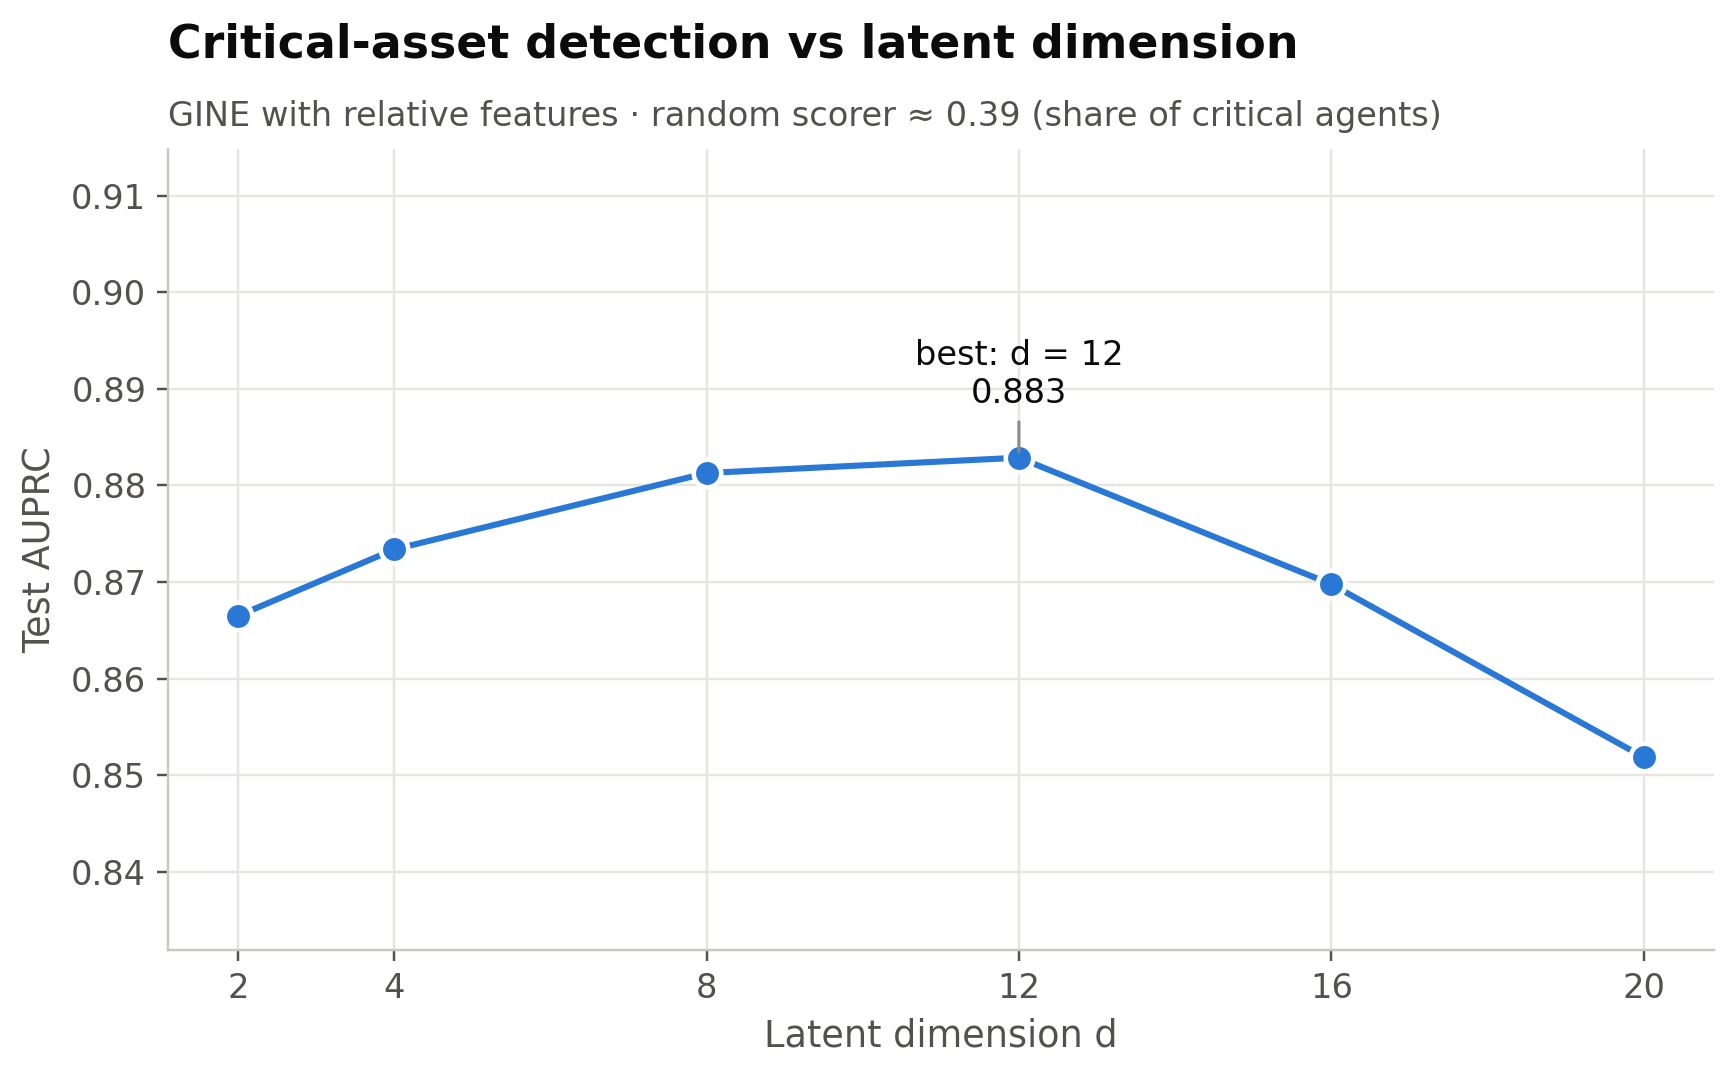
\includegraphics[width=\linewidth]{test_auprc_vs_d.png}\caption{E1: test AUPRC vs.\ $d$.}\end{subfigure}\hspace{0.04\textwidth}
\begin{subfigure}{0.40\textwidth}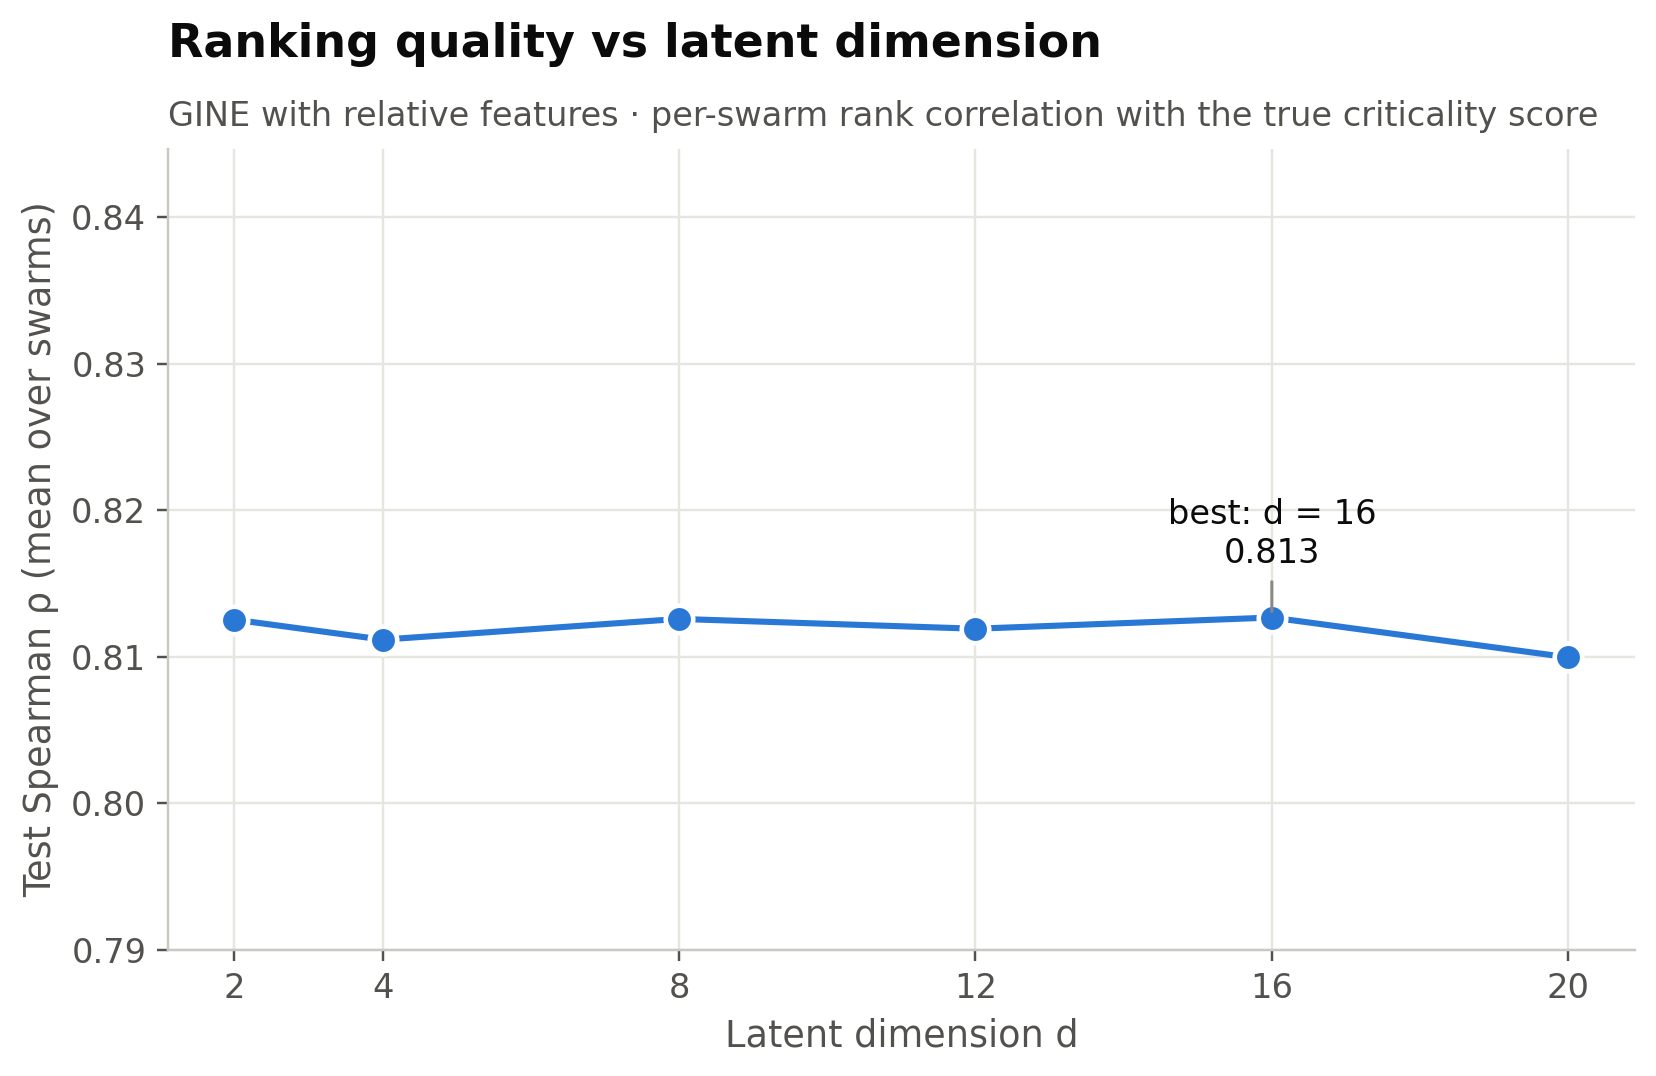
\includegraphics[width=\linewidth]{test_spearman_vs_d.png}\caption{E1: test $\rho$ vs.\ $d$.}\end{subfigure}\\[3pt]
\begin{subfigure}{0.56\textwidth}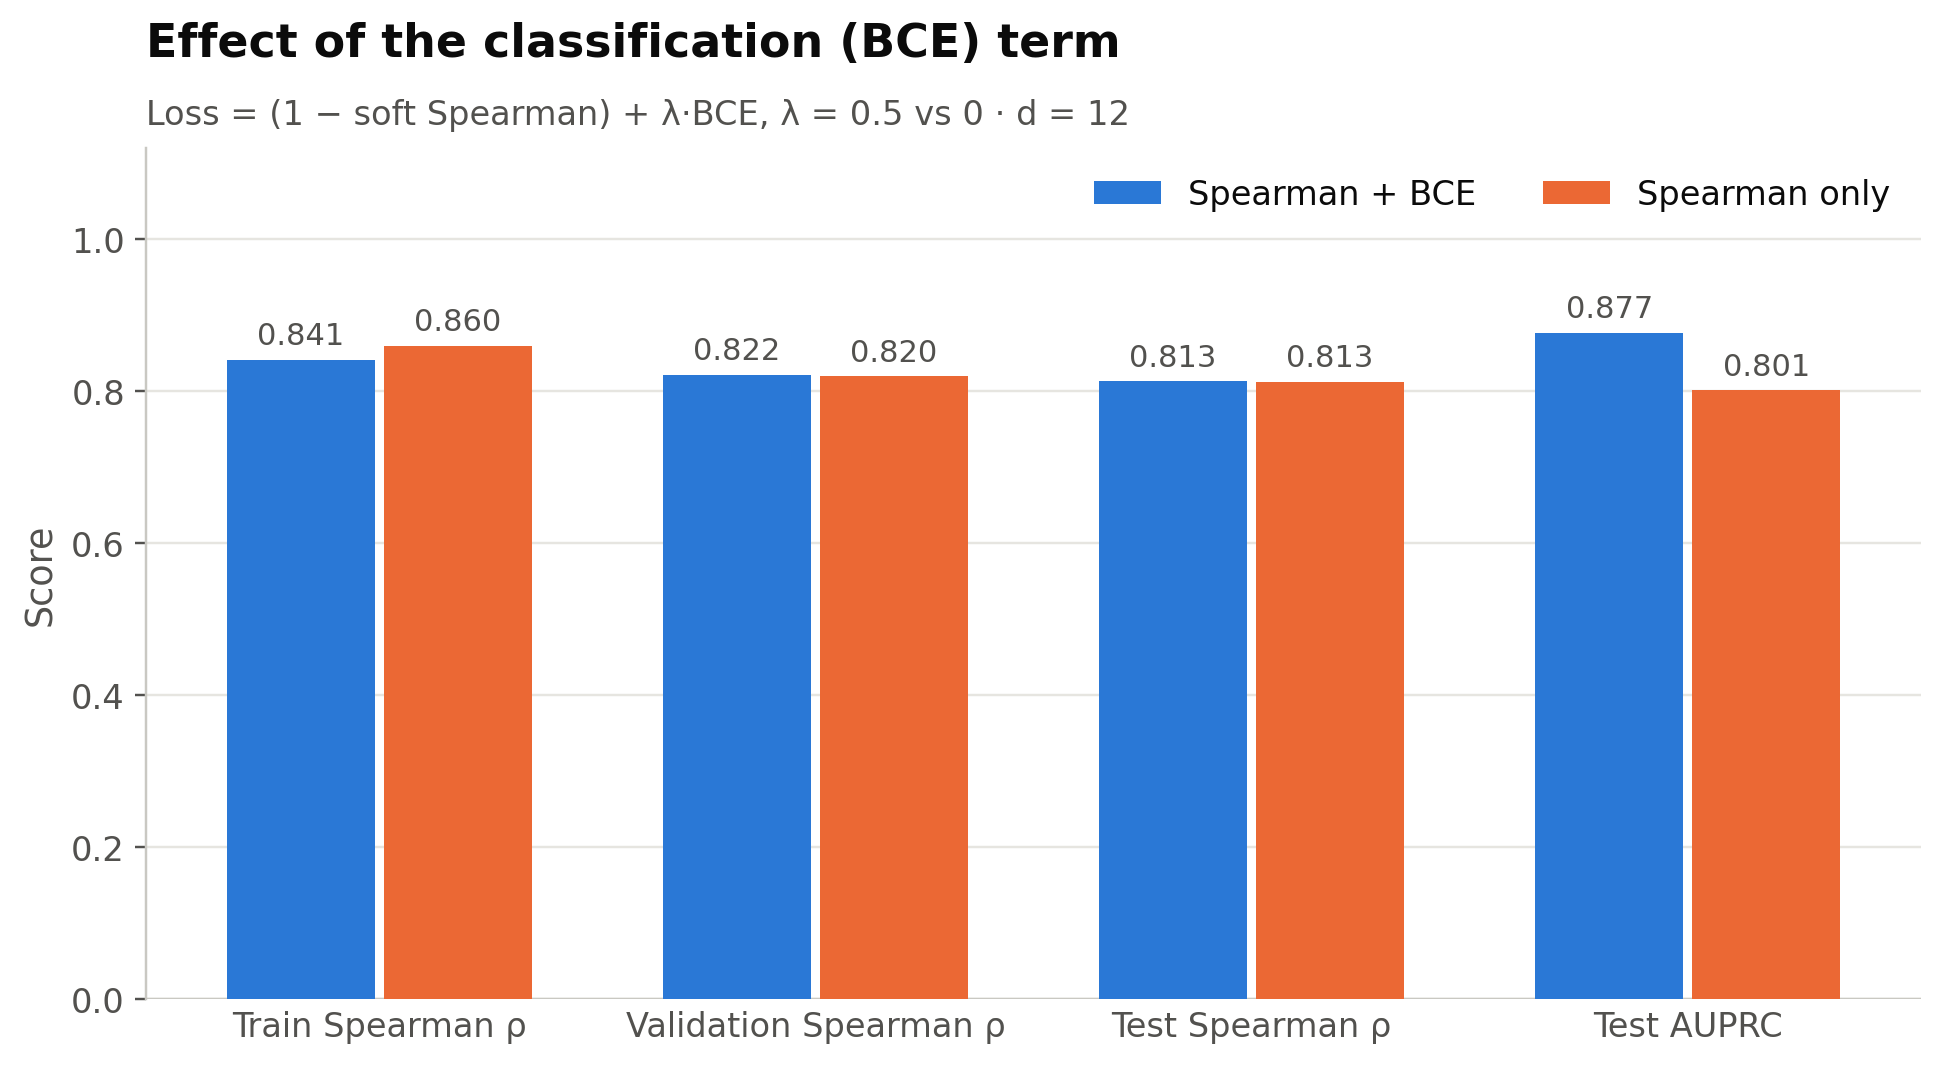
\includegraphics[width=\linewidth]{bce_ablation_metrics_d12.png}\caption{E3: with ($\lambda=0.5$) and without ($\lambda=0$) the classification term.}\end{subfigure}
\caption{Design-choice experiments. (a, b) Detection is best at $d=12$, while the test ranking changes by less than 0.004 across all latent
sizes. (c) Removing the classification term leaves the test ranking unchanged ($\rho=0.813$) but lowers AUPRC from 0.877 to 0.801, so the
term mainly improves detection and acts as a regulariser.}\label{fig:design}
\end{figure}

\begin{itemize}
\item \textbf{Latent size (E1).} Changing $d$ from 2 to 20 barely changes ranking performance: test $\rho$ remains
between 0.810 and 0.813. Classification is more sensitive. AUPRC increases from 0.866 for $d=2$ to 0.883 at
$d=12$, then decreases to 0.852 at $d=20$ (Figure~\ref{fig:design}a). This suggests that a small embedding is
enough to order the agents, but a little more capacity helps decide which ones are critical. The decline at larger
$d$ could be due to overfitting, since there are only 17 training swarms. I selected $d=12$.
\item \textbf{Relative features (E2).} Including the 11 within-swarm $z$-scores does not give a clear improvement:
the differences are about the same size as the variation across runs. A possible reason is that the swarm readout
already gives every agent information about the other agents. At $d=16$, the test $\rho$ values were 0.815 with
and 0.810 without the relative features (Appendix~\ref{app:d16}). The agent-level model benefited more clearly
($+0.022$ in test $\rho$). I kept these features in the final model because they are cheap to calculate and may
still help represent agents relative to their swarm.
\item \textbf{Classification term (E3).} Removing the classification term improves training rank correlation
(0.860 instead of 0.841), but both models reach 0.813 on the test set. The difference is much larger for detection:
AUPRC falls from 0.877 to 0.801 without the classification term. It therefore helps the model produce more useful
classification scores without harming the ranking. The train--test gap in $\rho$ also falls from 0.047 to 0.028.
The $d=16$ experiment gives a similar result, with AUPRC increasing from 0.774 to 0.874 when classification is included
(Appendix~\ref{app:d16}).

\end{itemize}

\FloatBarrier
\subsection{Overall performance and comparison with the baselines (E4)}\label{sec:overall}
Table~\ref{tab:overall} places the final model alongside the earlier Review~2 baselines and an agent-level GNN
from the final review. The agent-level GNN uses the same general network, but combines an agent's representations
over the full mission with additive attention and predicts one score for the whole agent rather than one score
at every timestep. The split and prediction task differ across some rows, so the table should not be treated
as a single controlled benchmark.

\begin{table}[!htbp]\centering\small
\caption{Test performance. Baselines and the Review~2 GNN are agent-level classifiers on the earlier, easier split (31/34/35 swarms,
fewer held-out conditions); the last three rows use the hard split of this report. The per-timestep model is scored per agent-timestep and, in the last row, per agent after averaging its scores over the mission.}\label{tab:overall}
\setlength{\tabcolsep}{3.6pt}\footnotesize
\begin{tabular}{@{}llccccccc@{}}\toprule
Model & Split & Acc. & Prec. & Recall & F1 & ROC-AUC & AUPRC & $\rho$\\\midrule
Logistic regression & Review 2 & 0.771 & 0.663 & 0.796 & 0.724 & 0.857 & 0.773 & ---\\
Gradient boosting & Review 2 & 0.887 & 0.881 & 0.808 & 0.843 & 0.957 & 0.933 & ---\\
GIN, classification only & Review 2 & 0.969 & 0.964 & 0.956 & 0.960 & 0.996 & 0.994 & ---\\\midrule
Agent-level GNN, $d=16$ & hard & 0.879 & 0.887 & 0.793 & 0.837 & 0.930 & 0.922 & 0.836\\
\textbf{Per-timestep GNN}, $d=12$ & hard & 0.822 & 0.748 & 0.810 & 0.778 & 0.900 & 0.873 & 0.816\\
\quad scores averaged over mission & hard & --- & --- & --- & --- & --- & \textbf{0.933} & \textbf{0.863}\\\bottomrule
\end{tabular}
\end{table}

\begin{figure}[!htbp]\centering
\begin{subfigure}[b]{0.36\textwidth}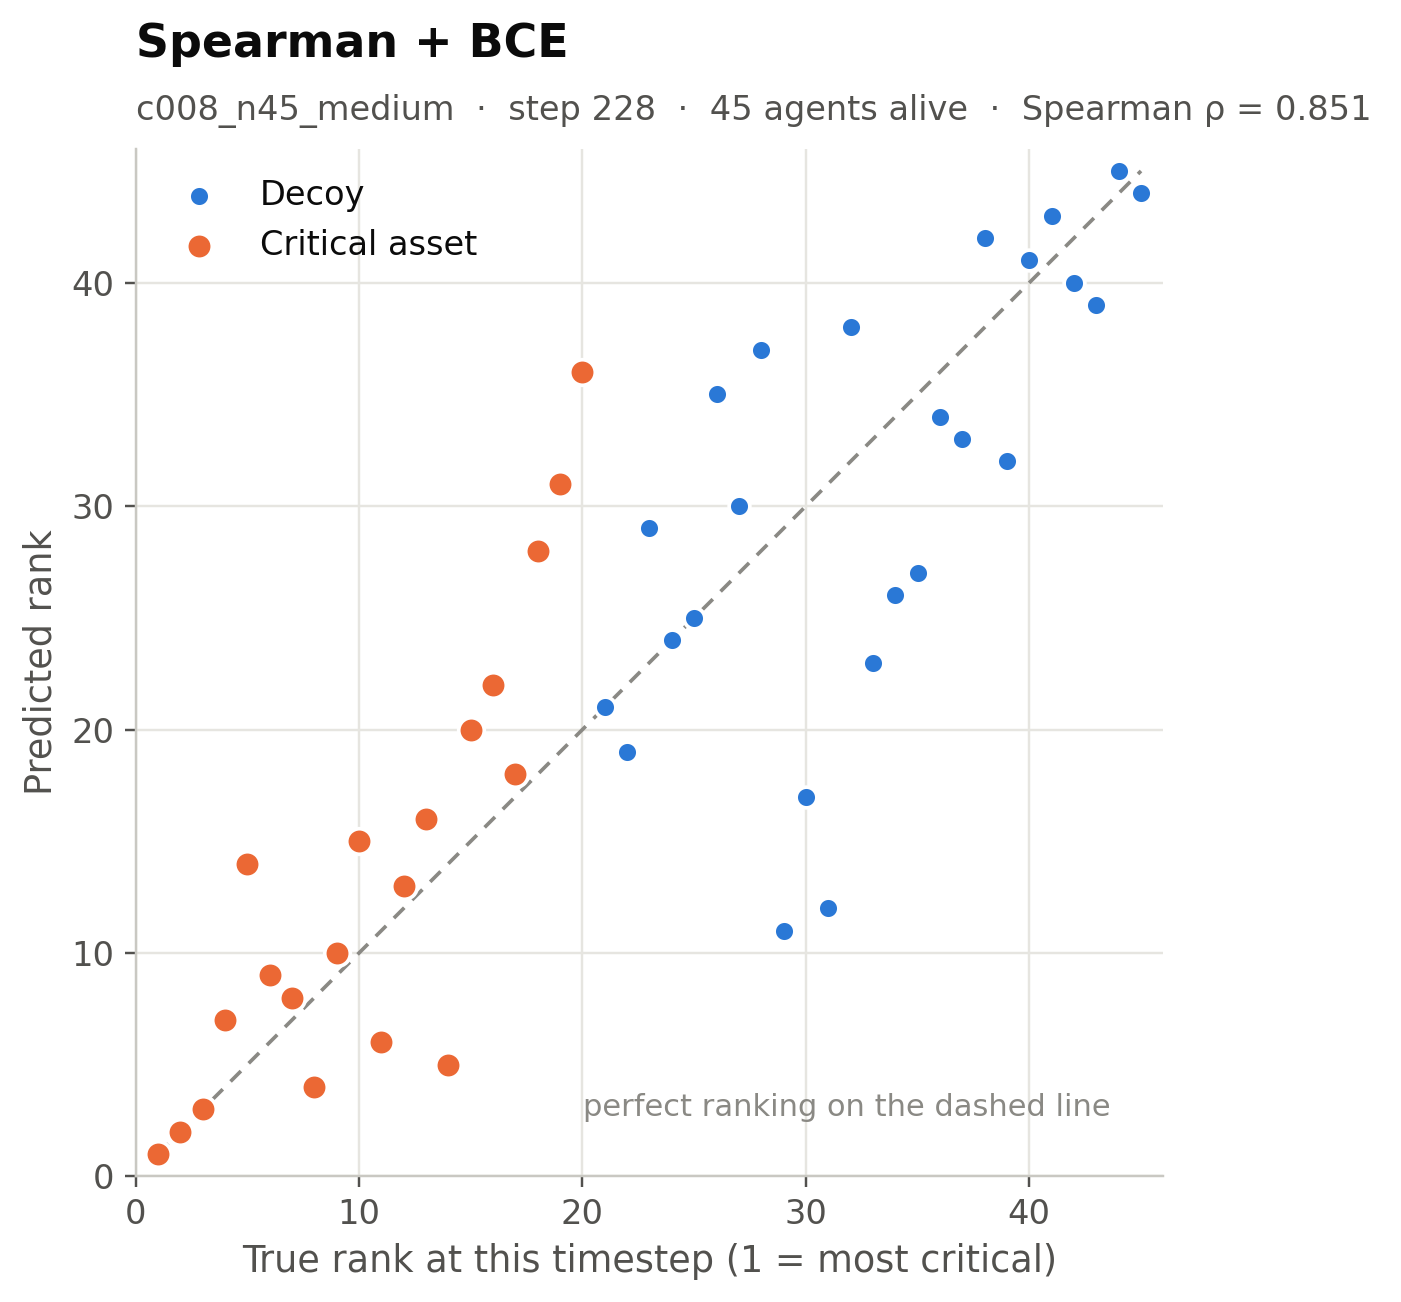
\includegraphics[width=\linewidth]{rank_example_final.png}\caption{True vs.\ predicted rank at one test step.}\end{subfigure}\hspace{0.03\textwidth}
\begin{subfigure}[b]{0.46\textwidth}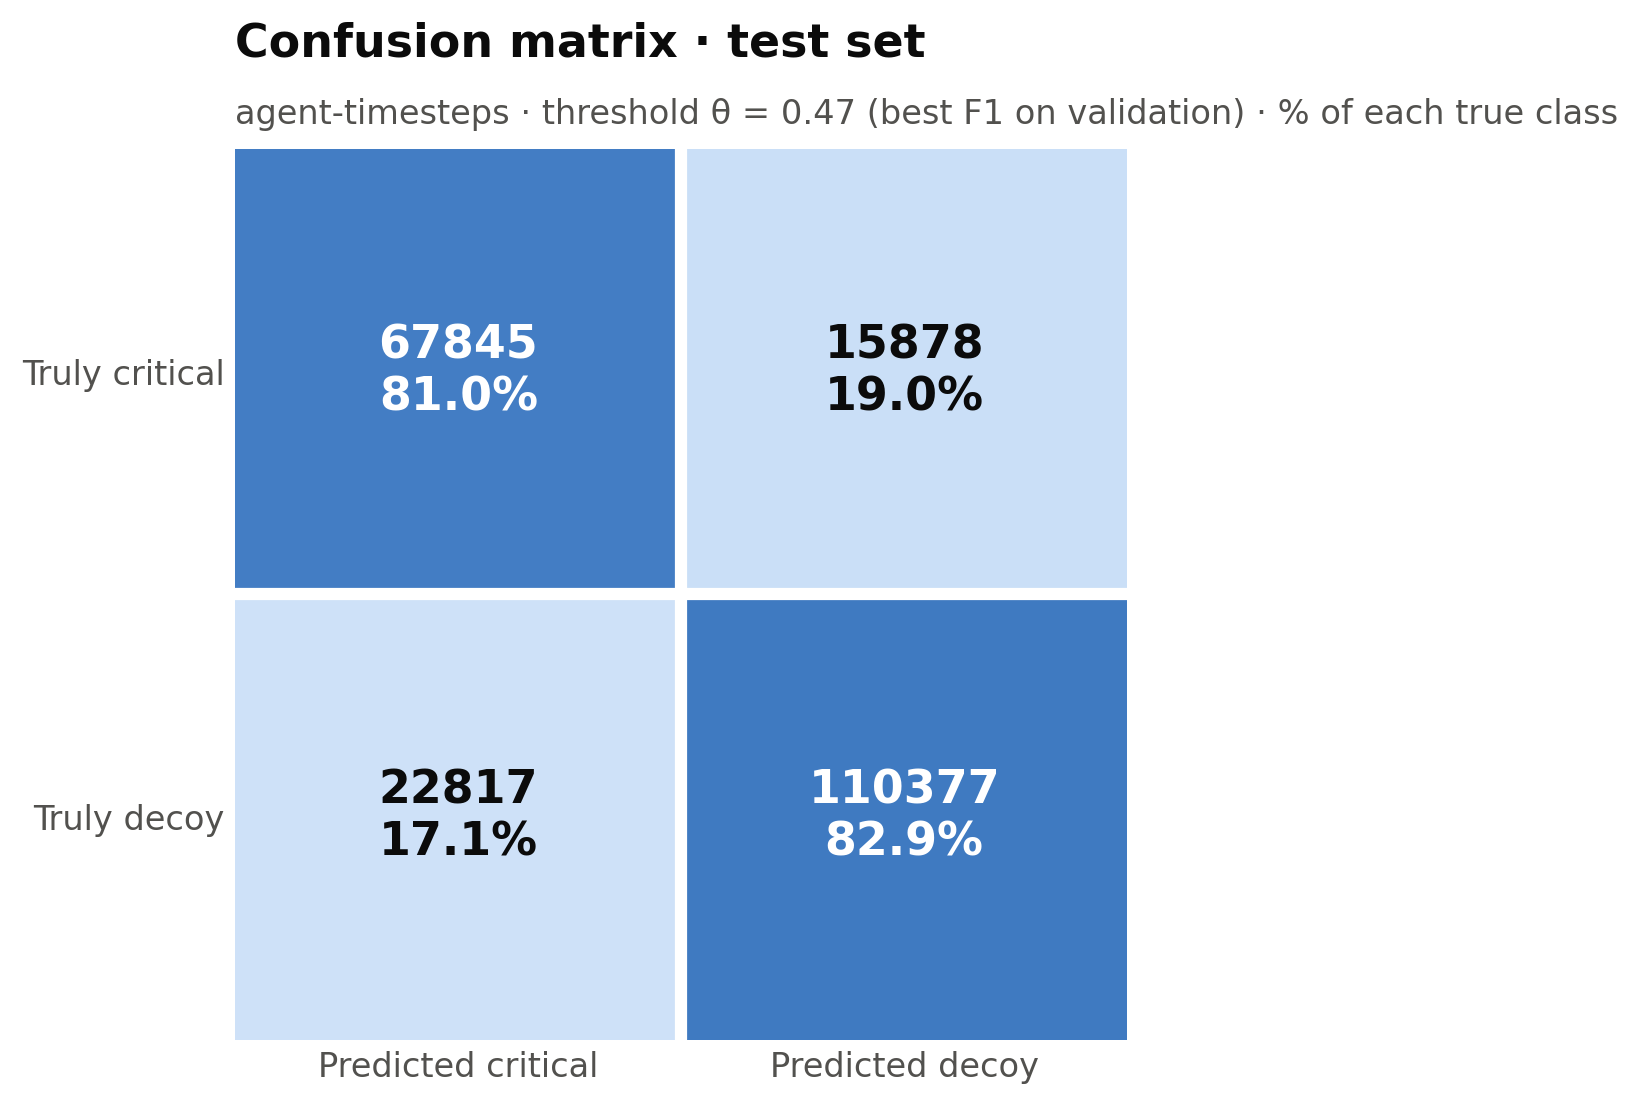
\includegraphics[width=\linewidth]{confusion_matrix_test.png}\caption{Test confusion matrix (agent-timesteps), $\theta=0.47$.}\end{subfigure}
\caption{Final model on the test set. (a) In a held-out swarm (45 agents, medium attrition) the ranking follows the diagonal
($\rho=0.85$) and most critical agents (orange) are placed in the top half. (b) About four in five critical agent-timesteps are detected,
and the errors are balanced between missed critical agents (19\,\%) and false alarms (17\,\%).}\label{fig:cm}
\end{figure}

\begin{itemize}
\item \textbf{Ranking and detection.} On the held-out test swarms, the model reaches a per-timestep Spearman
correlation of 0.816, Kendall $\tau$ of 0.675 and NDCG@10 of 0.809. Its AUPRC is 0.873, well above the random
baseline of 0.39, and ROC-AUC is 0.900. Validation and test ranking scores are quite close (0.823 and 0.816),
which is reassuring for the held-out conditions. At the validation-selected threshold $\theta=0.47$, it detects
81\,\% of the critical agent-timesteps and incorrectly flags 17\,\% of the non-critical ones
(Figure~\ref{fig:cm}).
\item \textbf{Comparison with earlier models.} I cannot directly compare these numbers with the Review~2
baselines because those models used entire trajectories and were tested on an easier split. For example, the
Review~2 GIN had AUPRC 0.994, but its only task was agent-level classification. On the harder split, the
agent-level GNN has AUPRC 0.922 and $\rho=0.836$. The per-timestep model has lower AUPRC (0.873), which is not
surprising because it must make a decision with only the current graph. However, if I average its scores for
each agent over the mission, the resulting agent-level evaluation gives $\rho=0.863$ and AUPRC 0.933. This is
encouraging, although it is not the same evaluation as making an online prediction at each step.

\end{itemize}

\FloatBarrier
\subsection{Behaviour over the mission (E4)}
\begin{figure}[!htbp]\centering
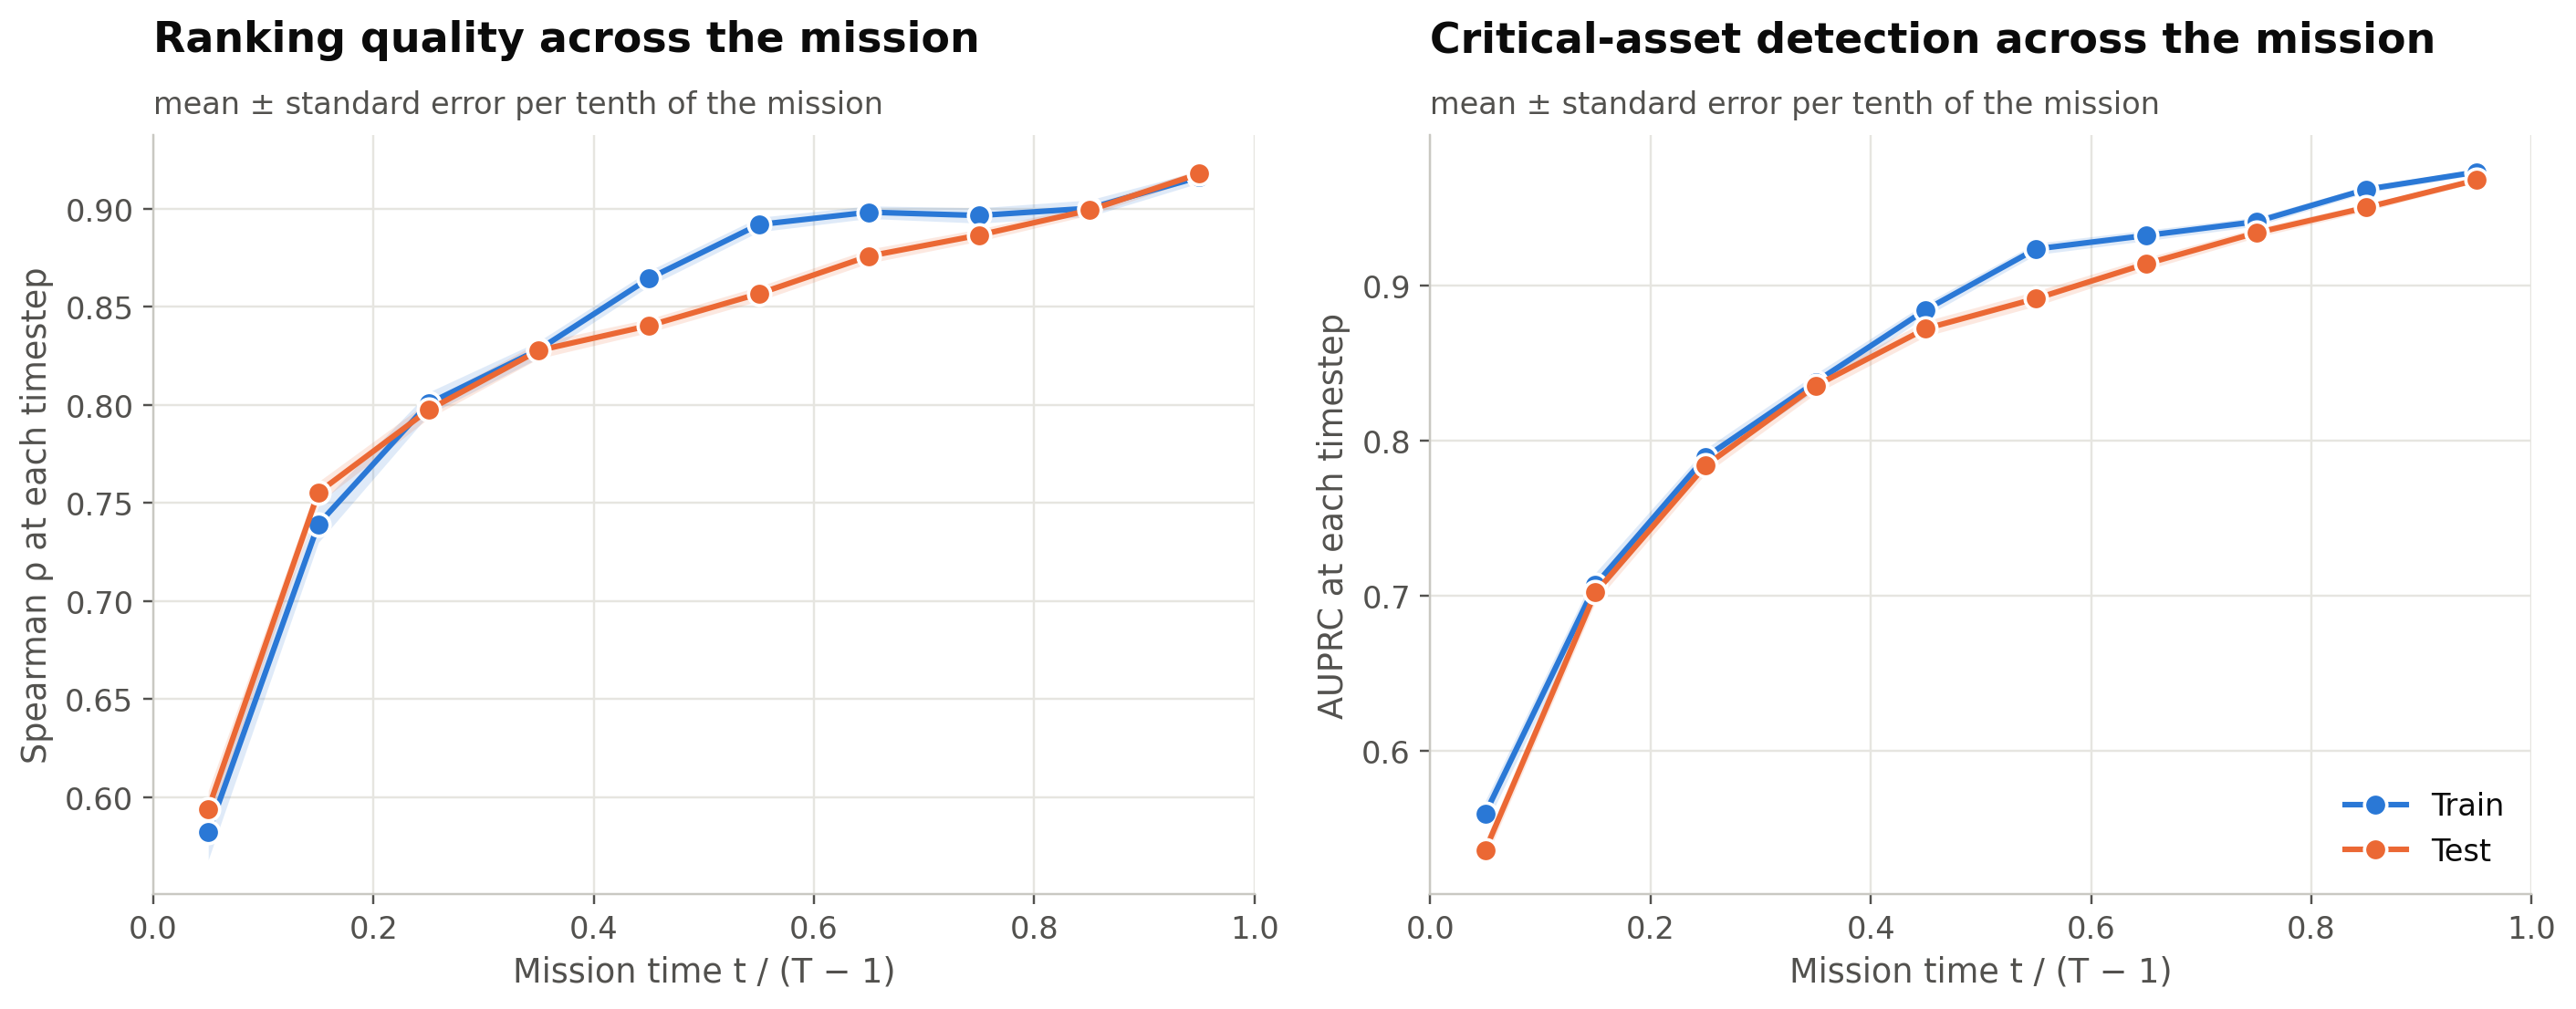
\includegraphics[width=0.88\textwidth]{performance_over_mission_time.png}
\caption{Ranking (left) and detection (right) performance over the course of a mission; each point is the mean over all timesteps in one tenth of the mission, with $\pm1$ standard error. Both metrics improve steadily (test $\rho$ from 0.59 to 0.92), and the training and test curves almost coincide, so the weaker early-mission performance is a property of the problem rather than over-fitting.}\label{fig:time}
\end{figure}

The average test score does not tell the whole story. Figure~\ref{fig:time} shows that in the first tenth of a
mission, test $\rho$ is only 0.59 and AUPRC is 0.54. By the last tenth they increase to 0.92 and 0.97.
The training curves follow almost the same pattern. From the example in Figure~\ref{fig:heat}a, the critical
agents tend to have lower and less clearly separated scores early in the mission. This makes it harder to infer
the correct order from just one graph. Later, their importance is more apparent from the current swarm
configuration. Since the same pattern appears in training and testing, I do not think it is simply a test-set
overfitting issue.

\begin{figure}[!htbp]\centering
\begin{subfigure}[b]{0.63\textwidth}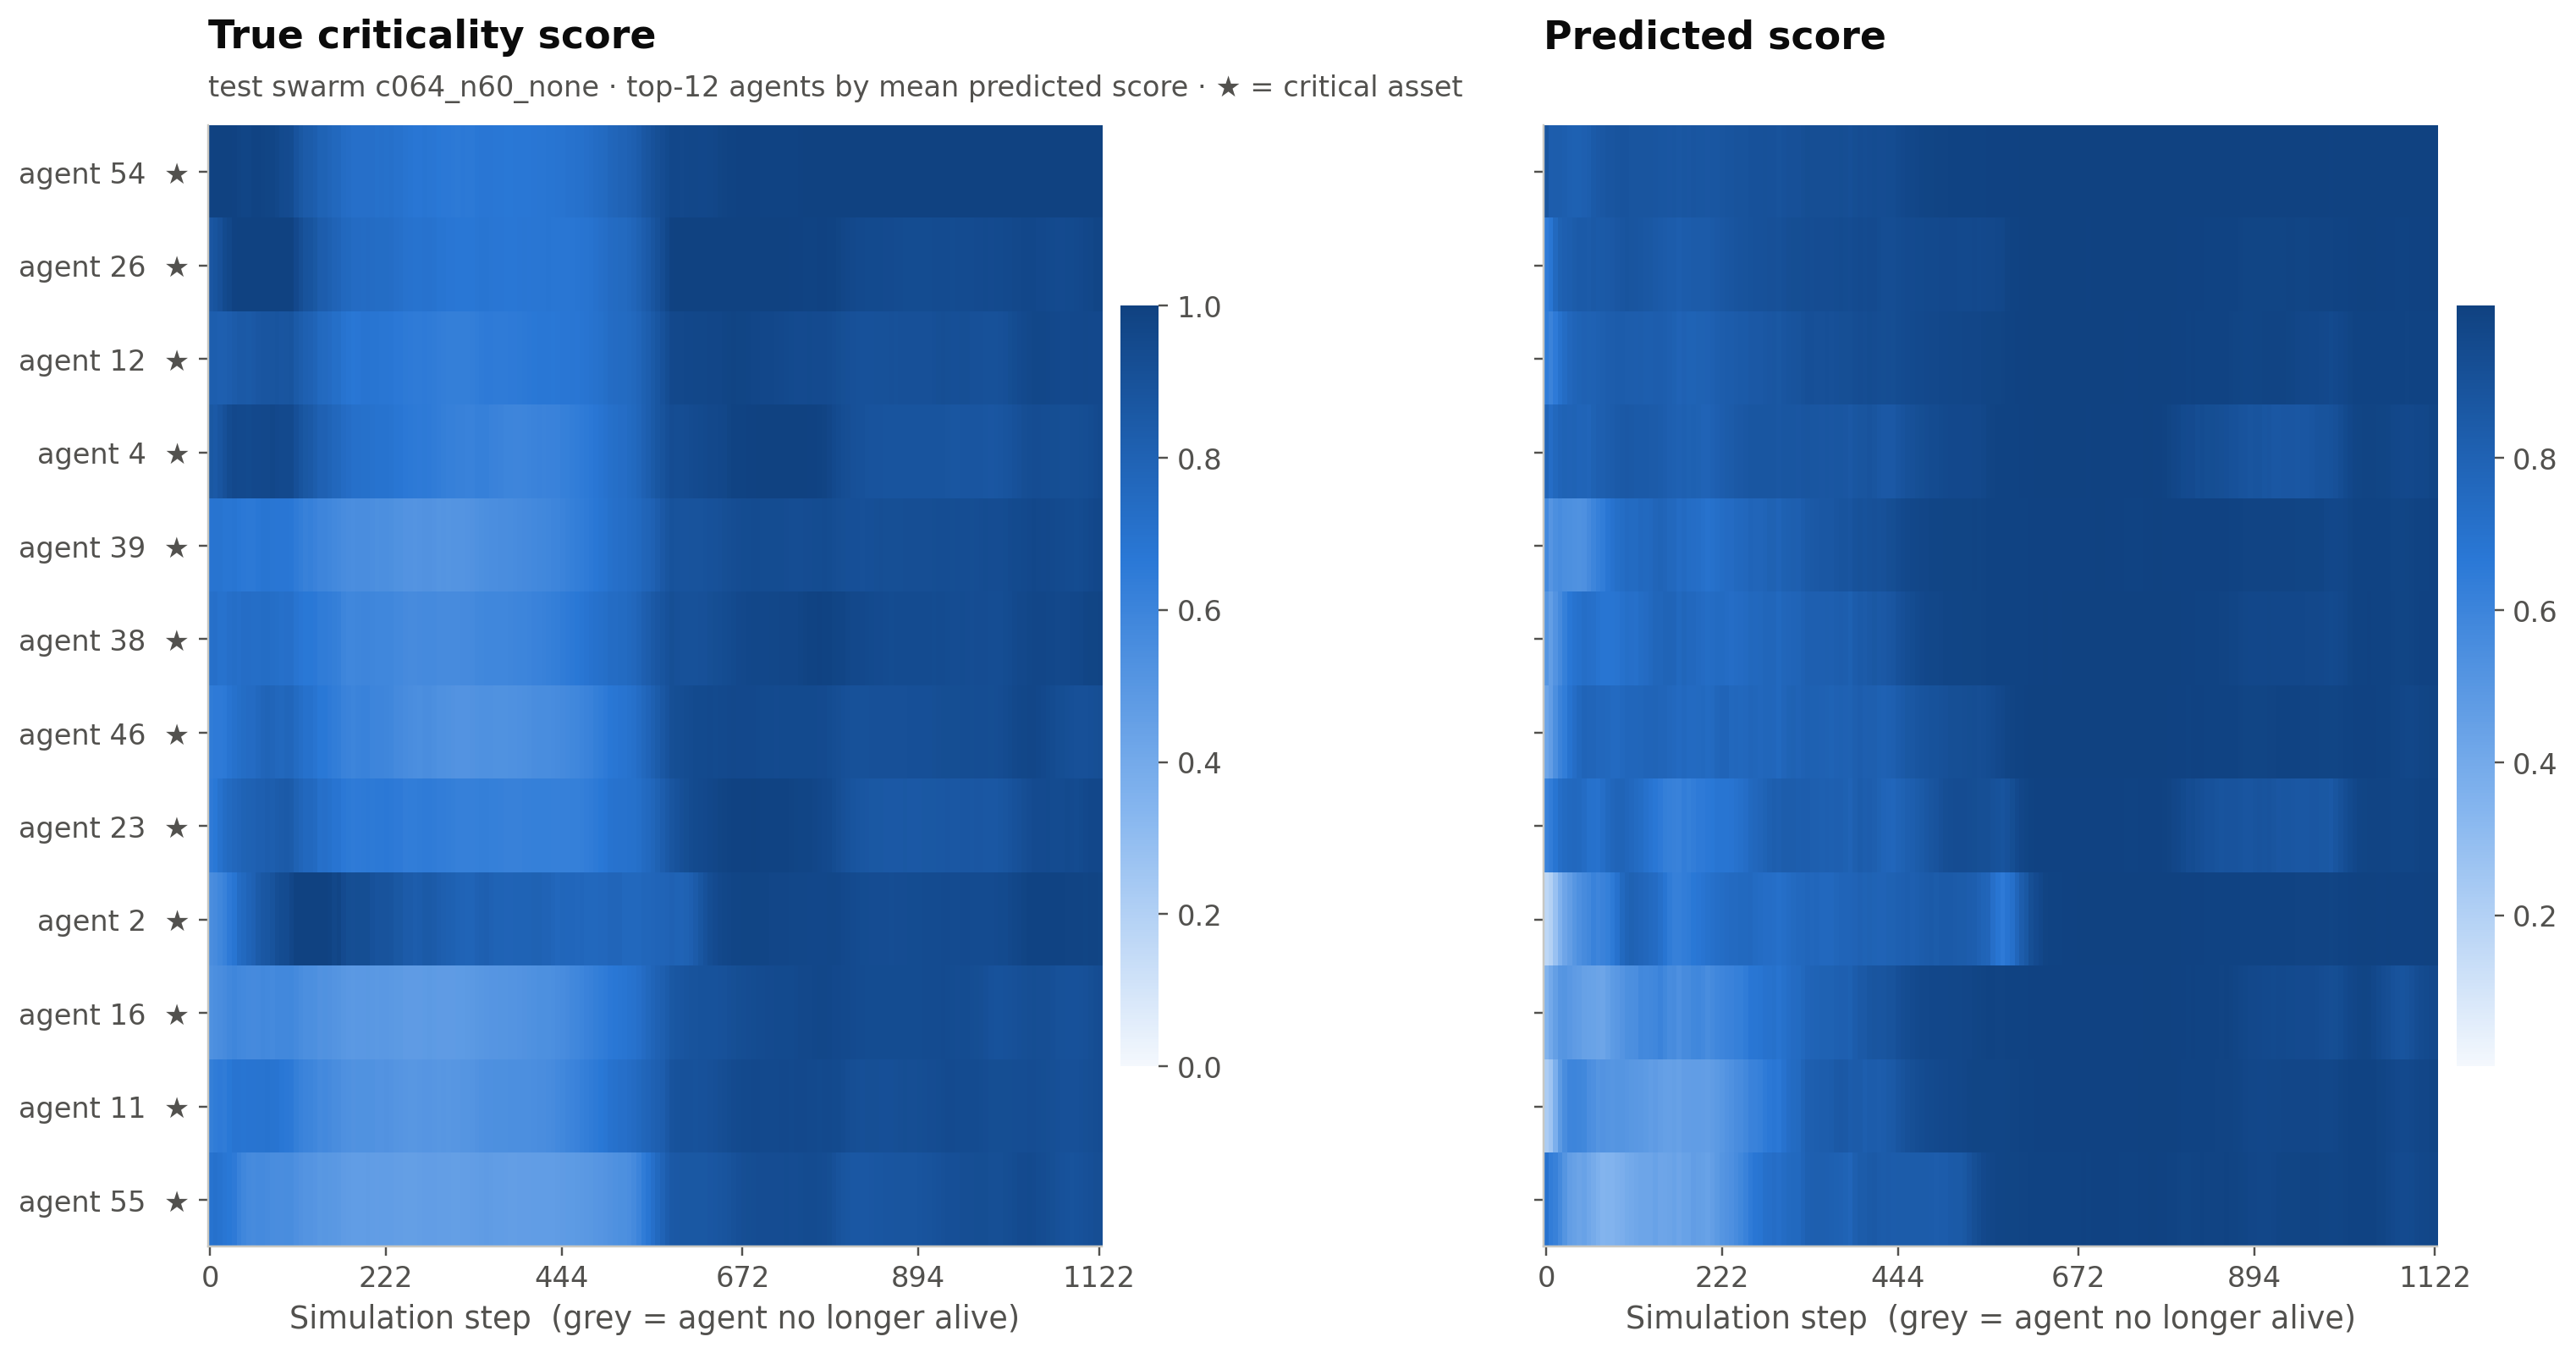
\includegraphics[width=\linewidth]{criticality_over_time_example.png}\caption{True (left) and predicted (right) scores of the 12 top-ranked agents of a test swarm; $\bigstar$ = critical.}\end{subfigure}\hfill
\begin{subfigure}[b]{0.35\textwidth}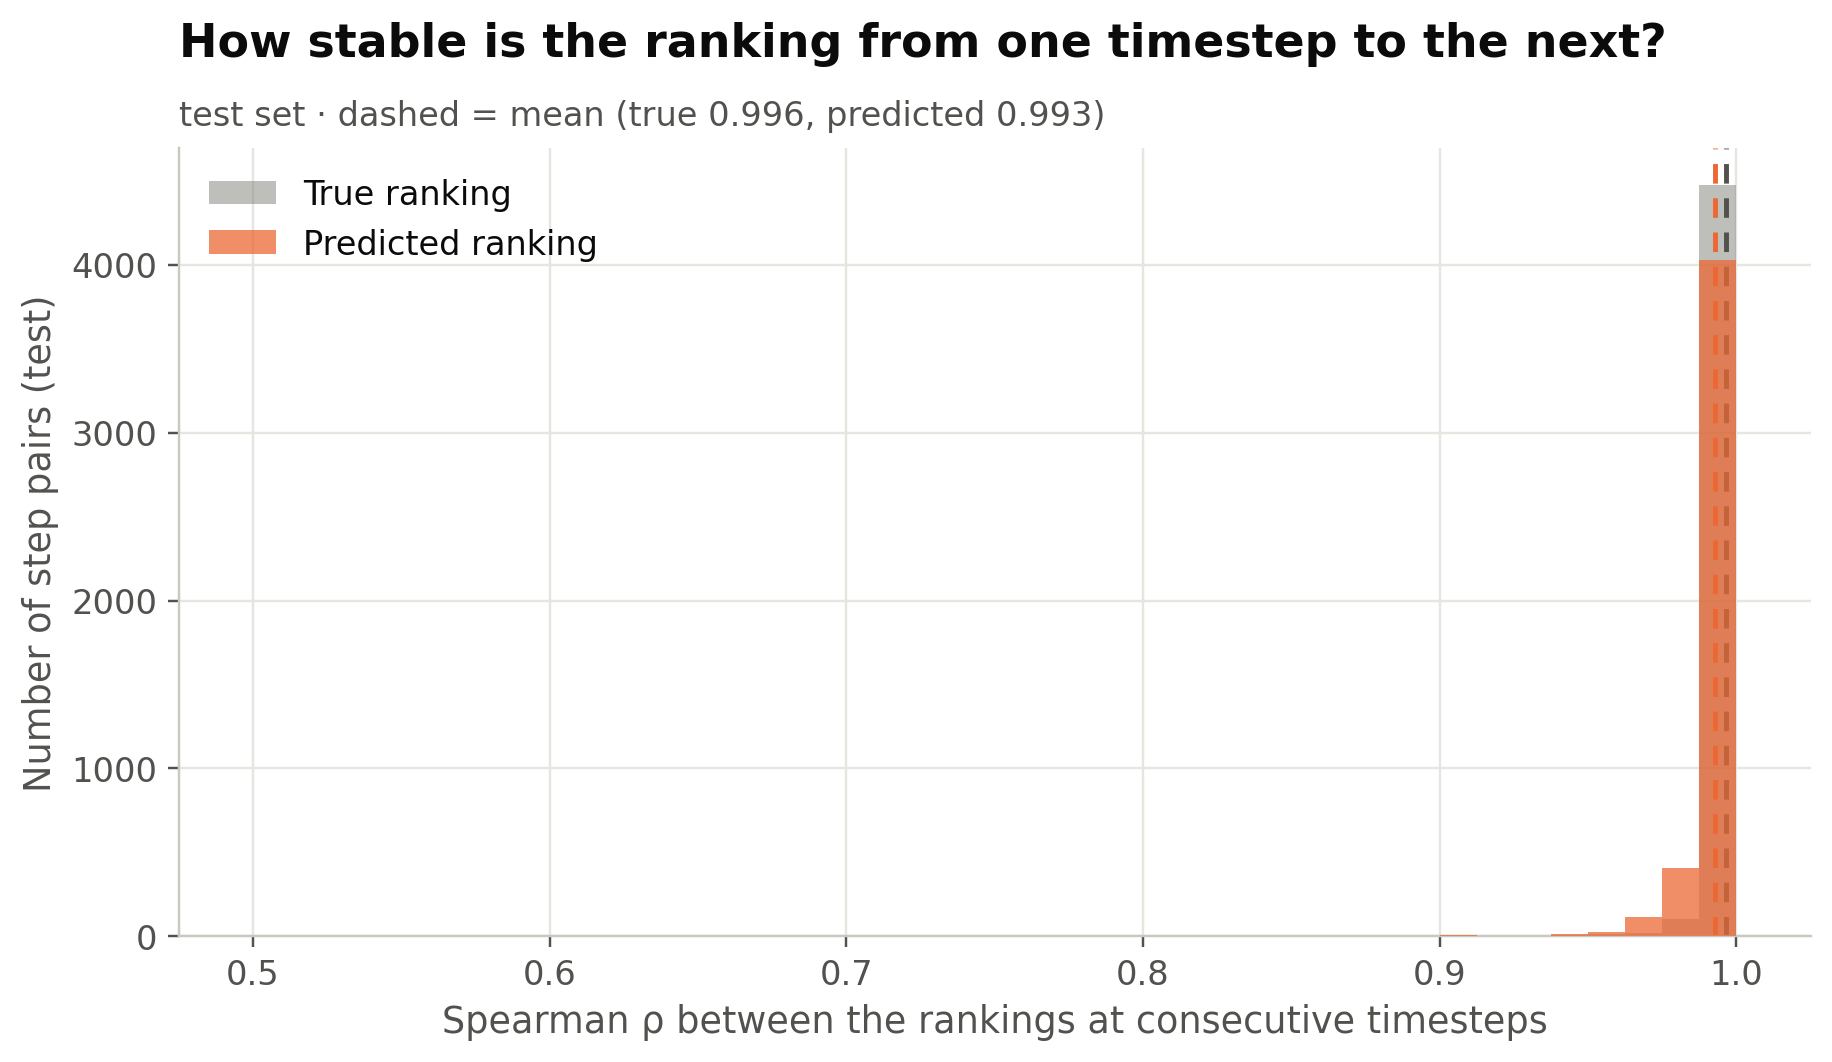
\includegraphics[width=\linewidth]{temporal_consistency_test.png}\caption{Spearman $\rho$ between the rankings at consecutive steps (test).}\end{subfigure}
\caption{Temporal behaviour of the predictions. (a) The predicted scores follow the rise in true criticality in the second half of the
mission, but several critical agents are under-scored in the first third. (b) Although every step is scored independently, the predicted
ranking is almost as stable from one step to the next as the true ranking (mean 0.993 vs.\ 0.996).}\label{fig:heat}
\end{figure}

Even though I do not explicitly smooth predictions over time, the ranks change quite gradually. The average
Spearman correlation between predictions at consecutive sampled steps is 0.993, compared with 0.996 for the true
scores (Figure~\ref{fig:heat}b). This addresses the concern from Review~2 about unstable timestep predictions,
at least in the results I measured. It does not solve the early-mission problem, however: Figure~\ref{fig:heat}a
shows several agents that are labelled critical but are given low scores in the first part of the mission.

\FloatBarrier
\subsection{Generalisation across operating conditions (E4)}
\begin{figure}[!htbp]\centering
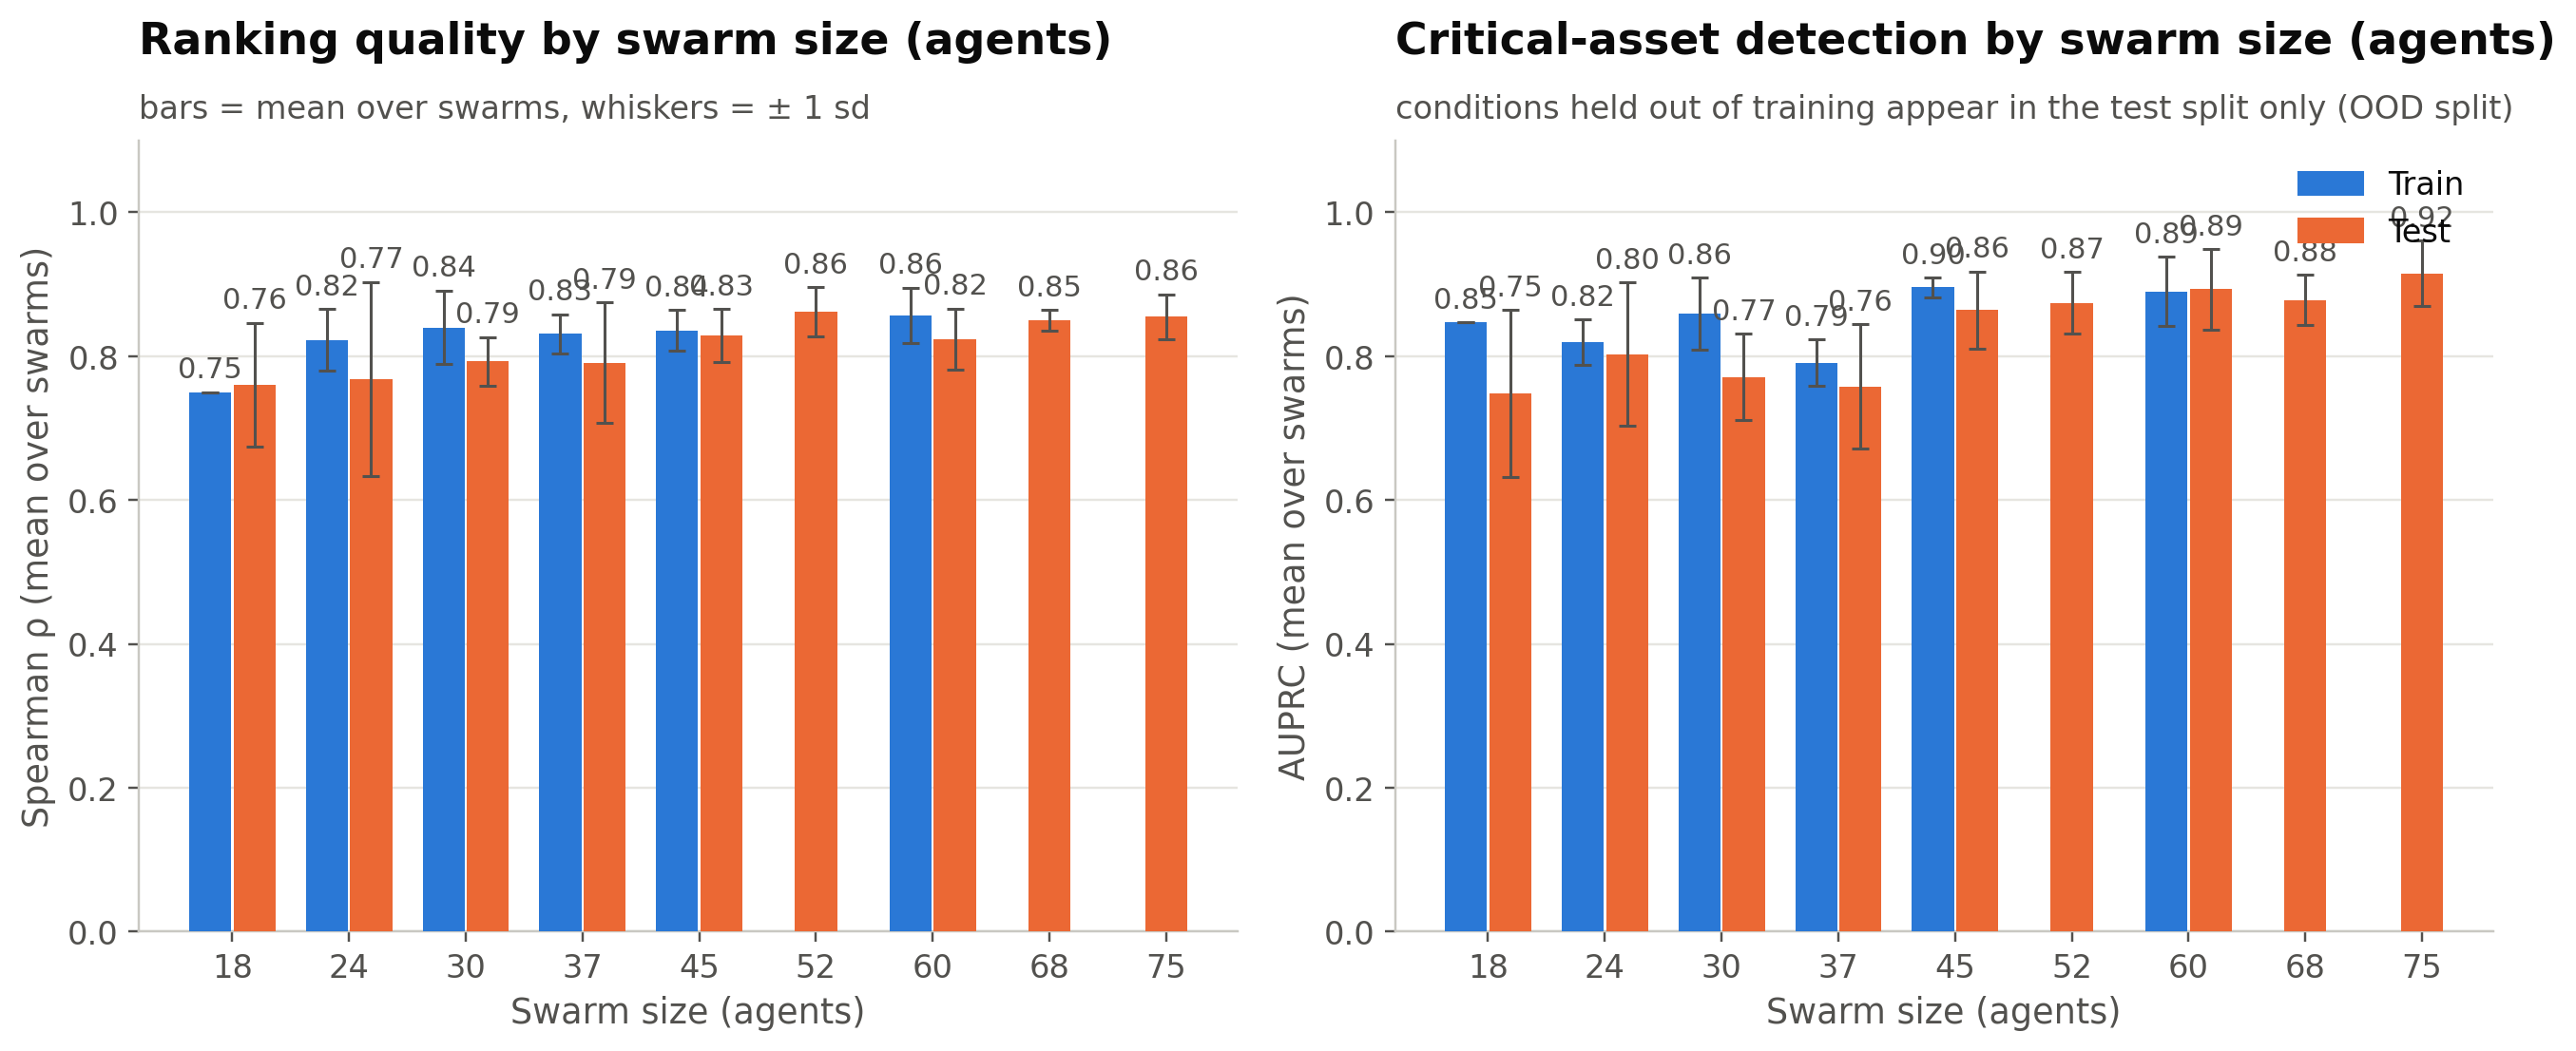
\includegraphics[width=0.80\textwidth]{performance_vs_num_agents.png}\\[2pt]
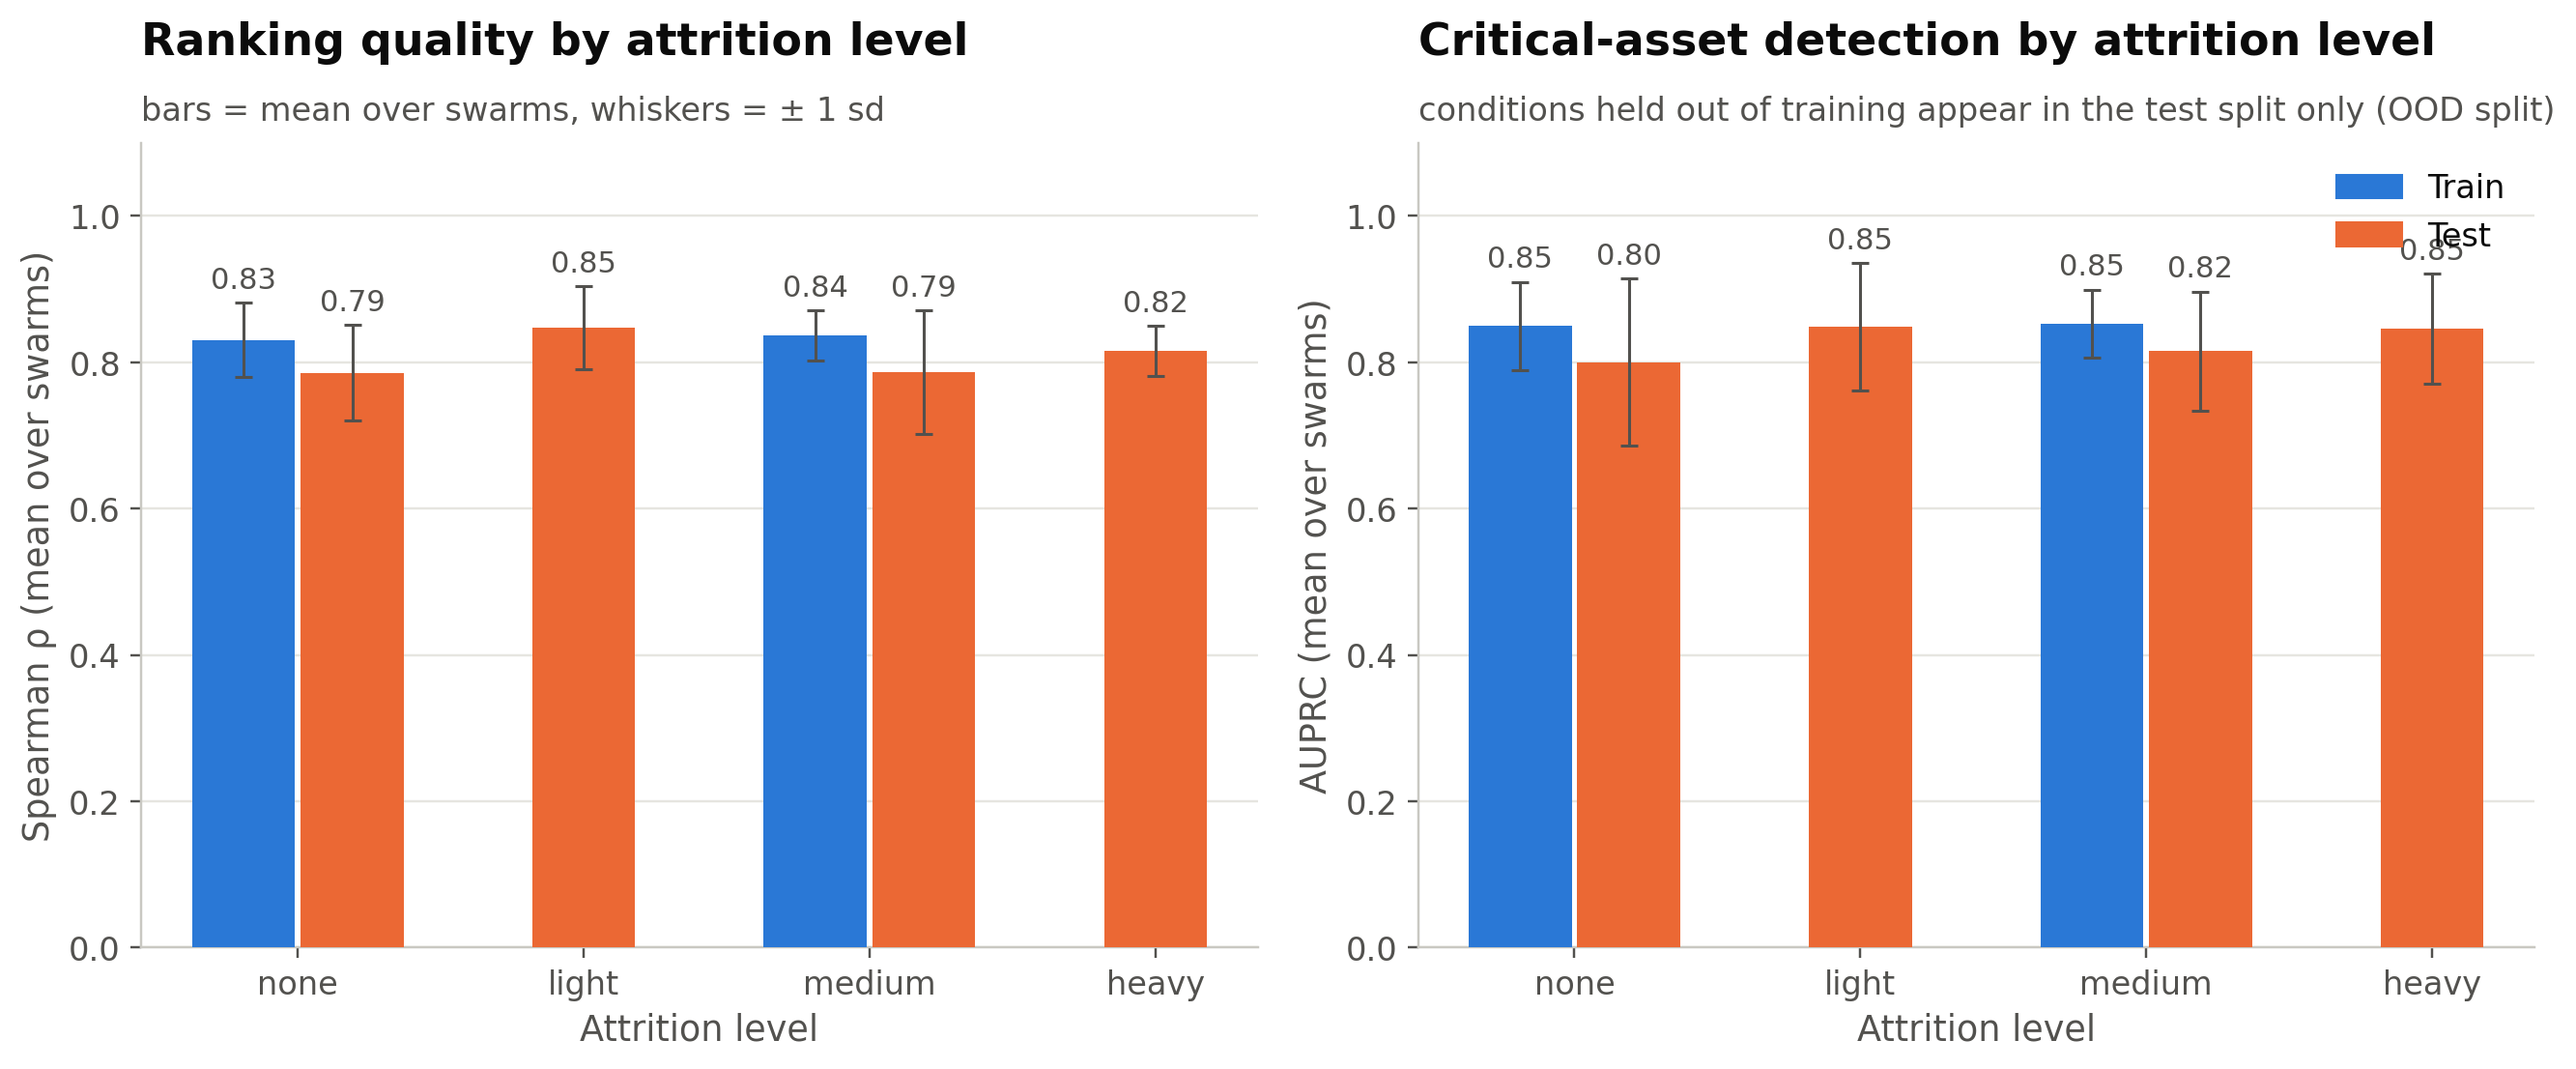
\includegraphics[width=0.80\textwidth]{performance_vs_attrition.png}\\[2pt]
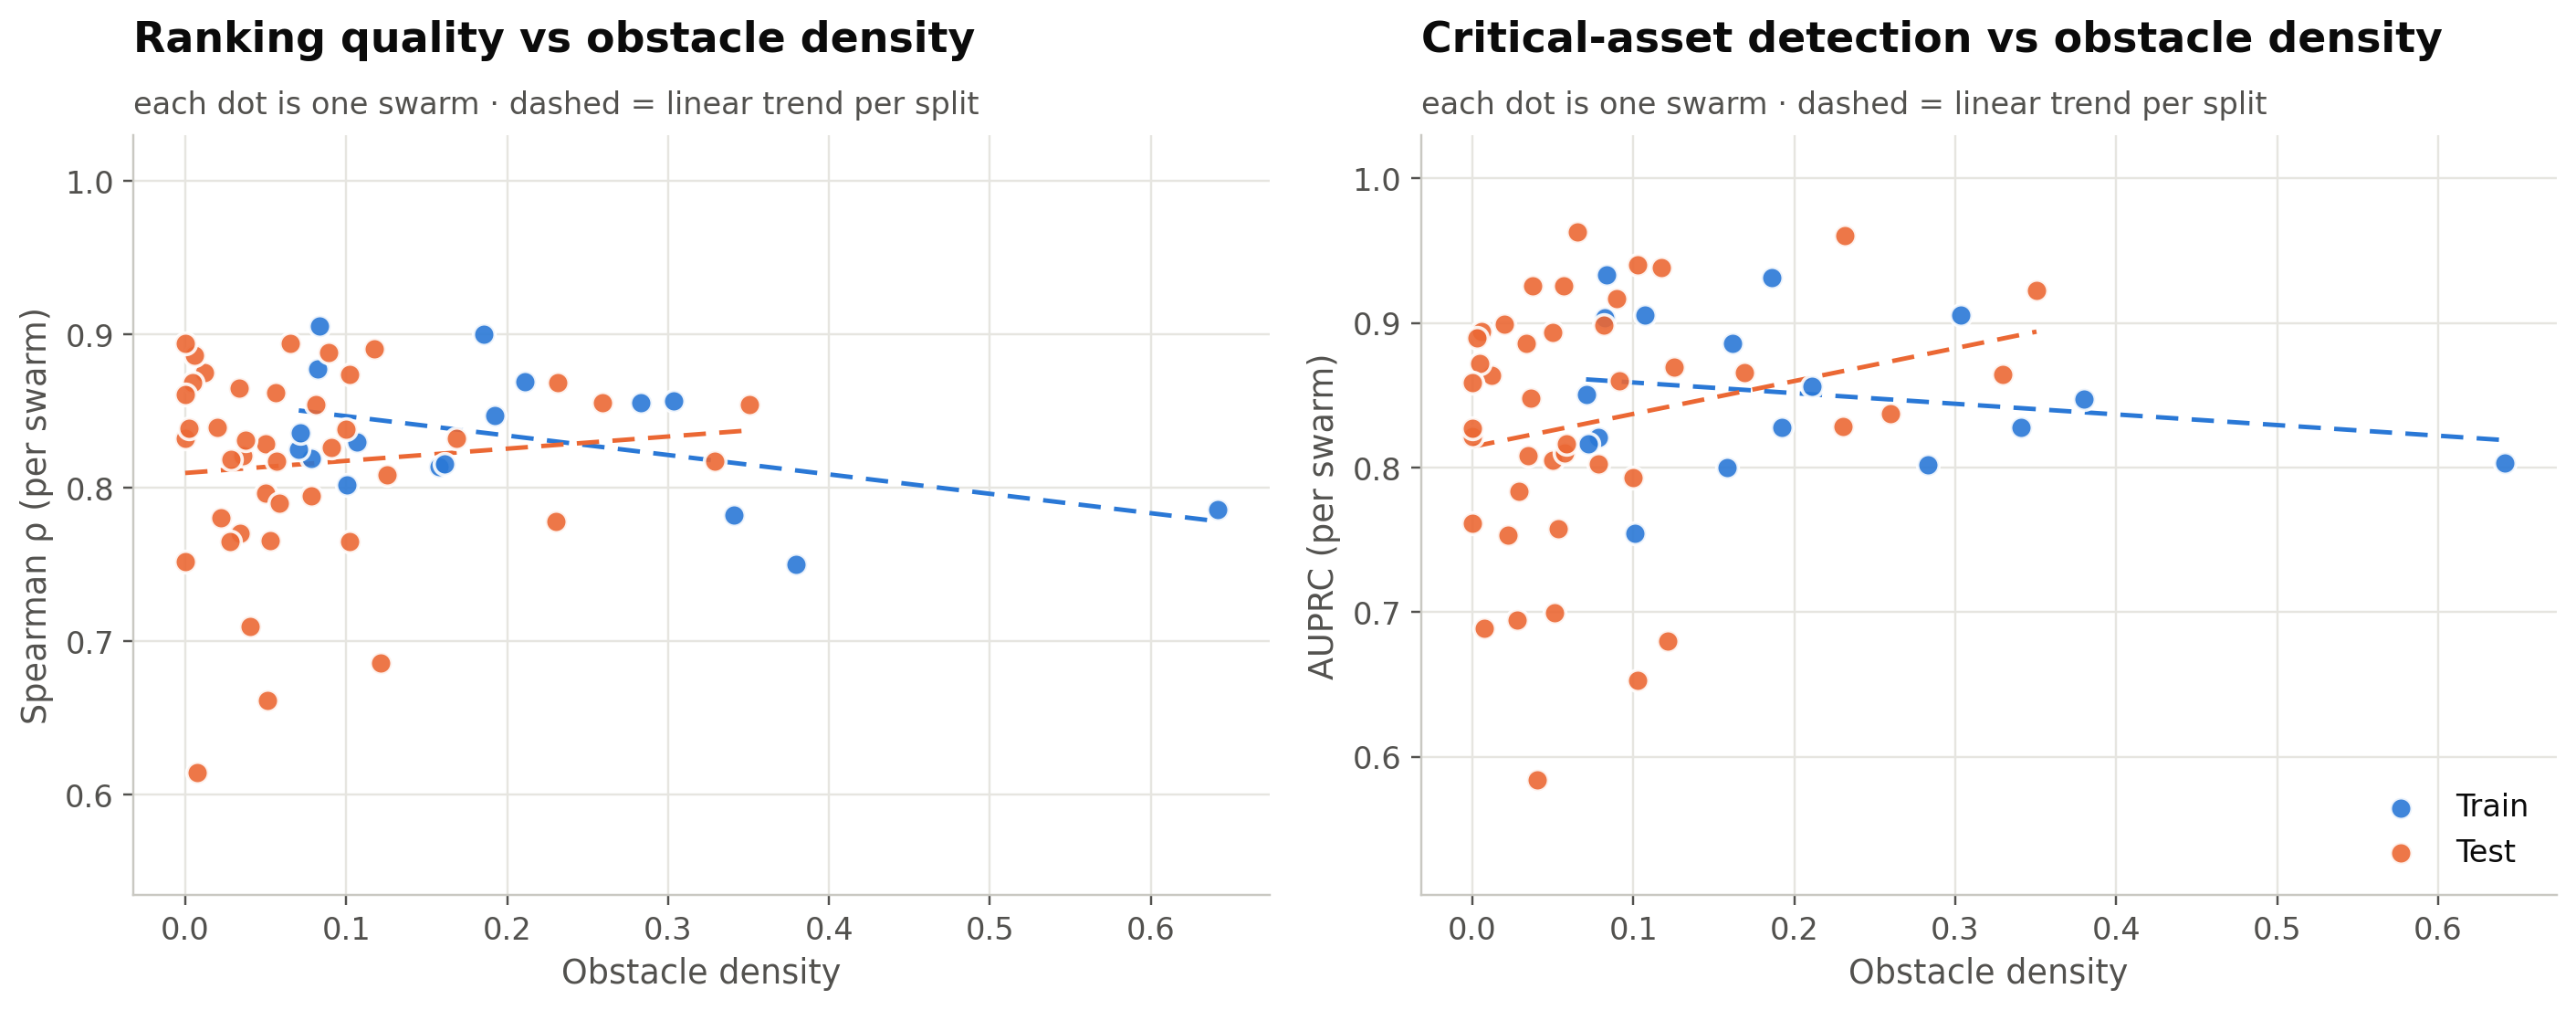
\includegraphics[width=0.80\textwidth]{performance_vs_obstacle_density.png}
\caption{Per-swarm Spearman correlation and AUPRC by swarm size (top), attrition level (middle) and obstacle density (bottom). Sizes 52, 68
and 75, light and heavy attrition and densities below 0.07 occur only in held-out swarms. Unseen sizes and attrition levels are handled as
well as the seen ones; the smallest swarms and the sparse-obstacle region (where the weakest test swarms lie) are the most difficult.}\label{fig:cond}
\end{figure}

\begin{itemize}
\item \textbf{Swarm size.} The model works reasonably well on sizes it did not see in training. For 52, 68 and
75 agents, the test $\rho$ values are 0.86, 0.85 and 0.86, with AUPRC values 0.87, 0.88 and 0.92
(Figure~\ref{fig:cond}, top). The model shares weights across nodes and uses a mean for the global readout,
so it is not tied to one fixed number of agents. Smaller swarms are more difficult: for 18 and 24 agents,
test $\rho$ is 0.76 and 0.77, and AUPRC is 0.75 and 0.80. A mistake in just a few ranks has a larger effect
when the swarm is small.
\item \textbf{Attrition.} The held-out light and heavy attrition cases give test $\rho$ values 0.85 and 0.82,
and both have AUPRC around 0.85. These results are at least comparable to the cases with no or medium attrition
($\rho\approx0.79$). Since some test cases are held out for more than one reason, this is not a perfectly
isolated experiment on attrition, but it suggests that the model can handle different levels of agent loss.
\item \textbf{Obstacles and clutter.} There is no obvious overall trend with obstacle density or clutter
(Figure~\ref{fig:cond}, bottom, and Appendix Figure~\ref{fig:obst}). Still, the weakest test swarms,
with $\rho$ around 0.61--0.66 and AUPRC as low as 0.58, occur in relatively sparse obstacle fields
(density below 0.13). The training cases all have density at least 0.07, so this is an area where the model
may not have enough varied examples.

\end{itemize}

\subsection{Which inputs the model relies on (E4)}\label{sec:features}
\begin{figure}[!htbp]\centering
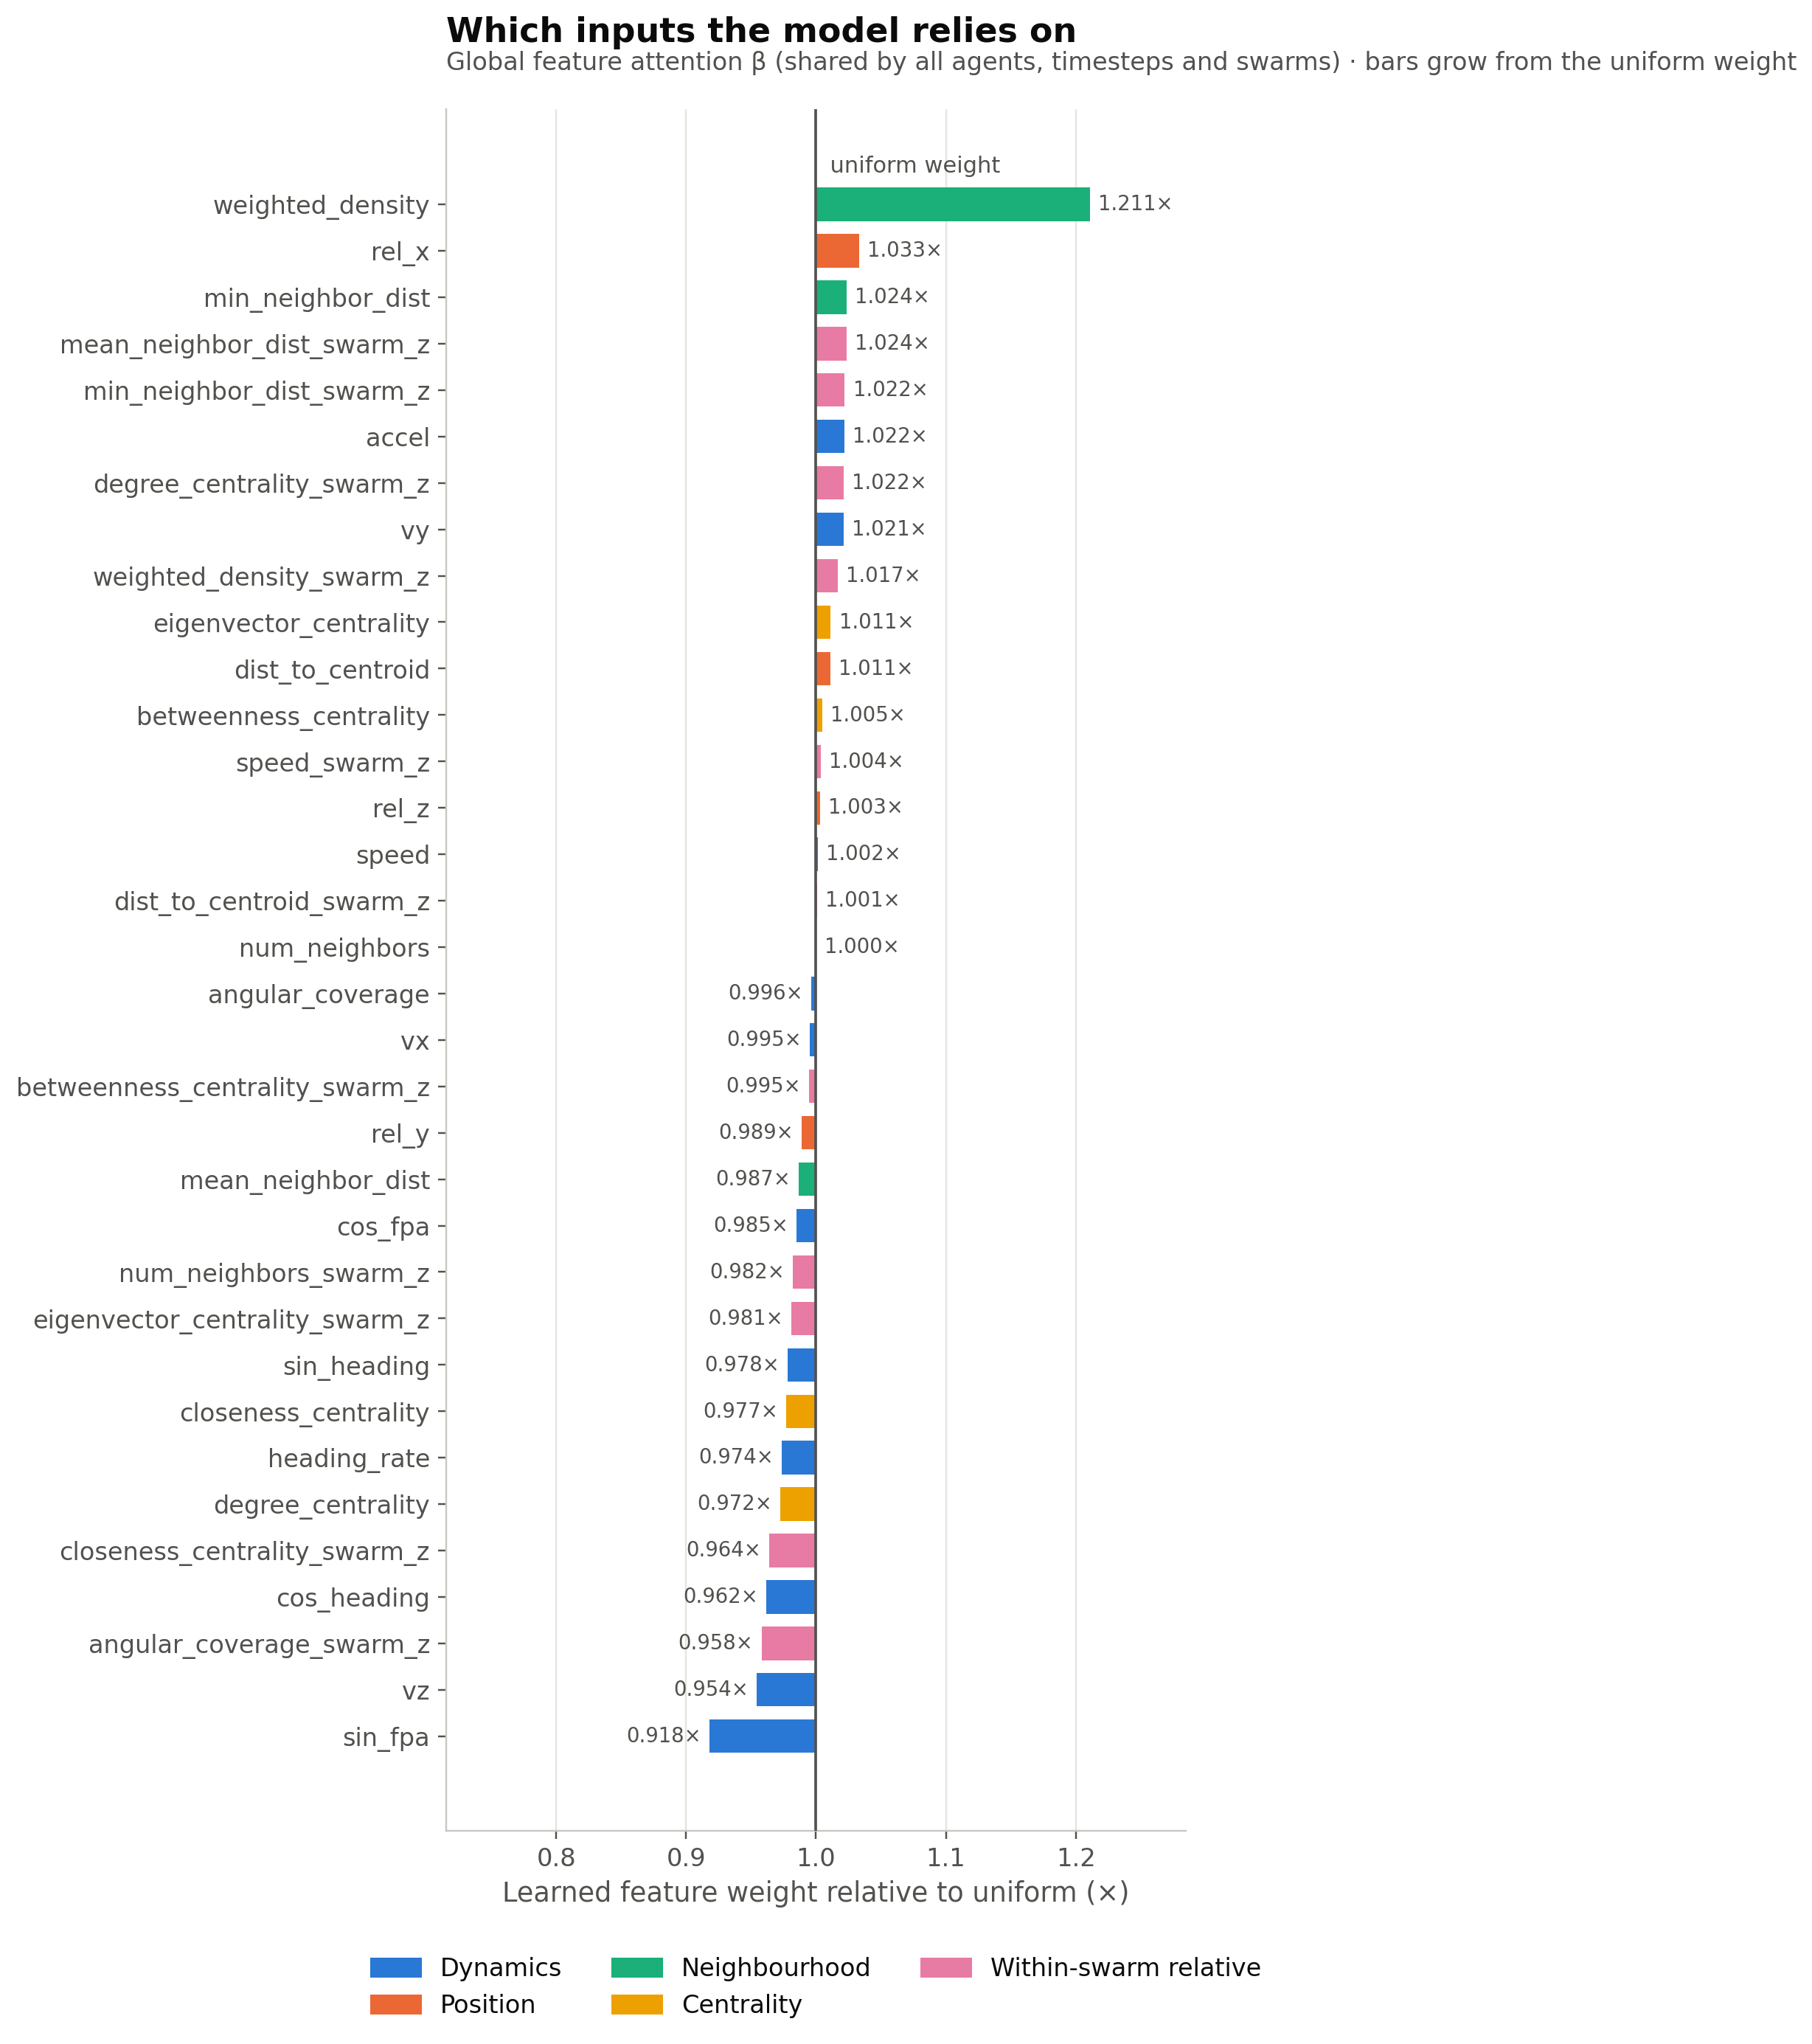
\includegraphics[width=0.50\textwidth]{feature_attention_weights.png}
\caption{Learned feature-attention weights relative to the uniform weight $1/34$, coloured by feature group. The distance-weighted local
density is weighted most (1.21$\times$), while vertical motion and heading are weighted least, indicating that criticality depends mainly
on how crowded an agent's neighbourhood is.}\label{fig:fa}
\end{figure}
Figure~\ref{fig:fa} shows the feature-attention weights, expressed relative to the uniform value $1/34$.
They range from 0.92 to 1.21 times that value. Distance-weighted local density has the largest weight
(1.21$\times$). The next few are much closer to uniform: relative $x$ position is 1.03$\times$, while the
minimum neighbour distance and two relative neighbour-distance features are about 1.02$\times$ each.
Among the smaller weights are $\sin$ of flight-path angle (0.92$\times$), $v_z$ (0.95$\times$) and
$\cos$ of heading (0.96$\times$).

This points towards neighbourhood geometry being more useful for the model than vertical motion or heading.
It also fits with the earlier observation that centrality features alone are not strong predictors.
However, these attention weights should not be interpreted as a causal feature-importance measure:
subsequent GINE layers can change the effective contribution of any input.

\subsection{Robustness to input noise (E5)}
\begin{figure}[!htbp]\centering
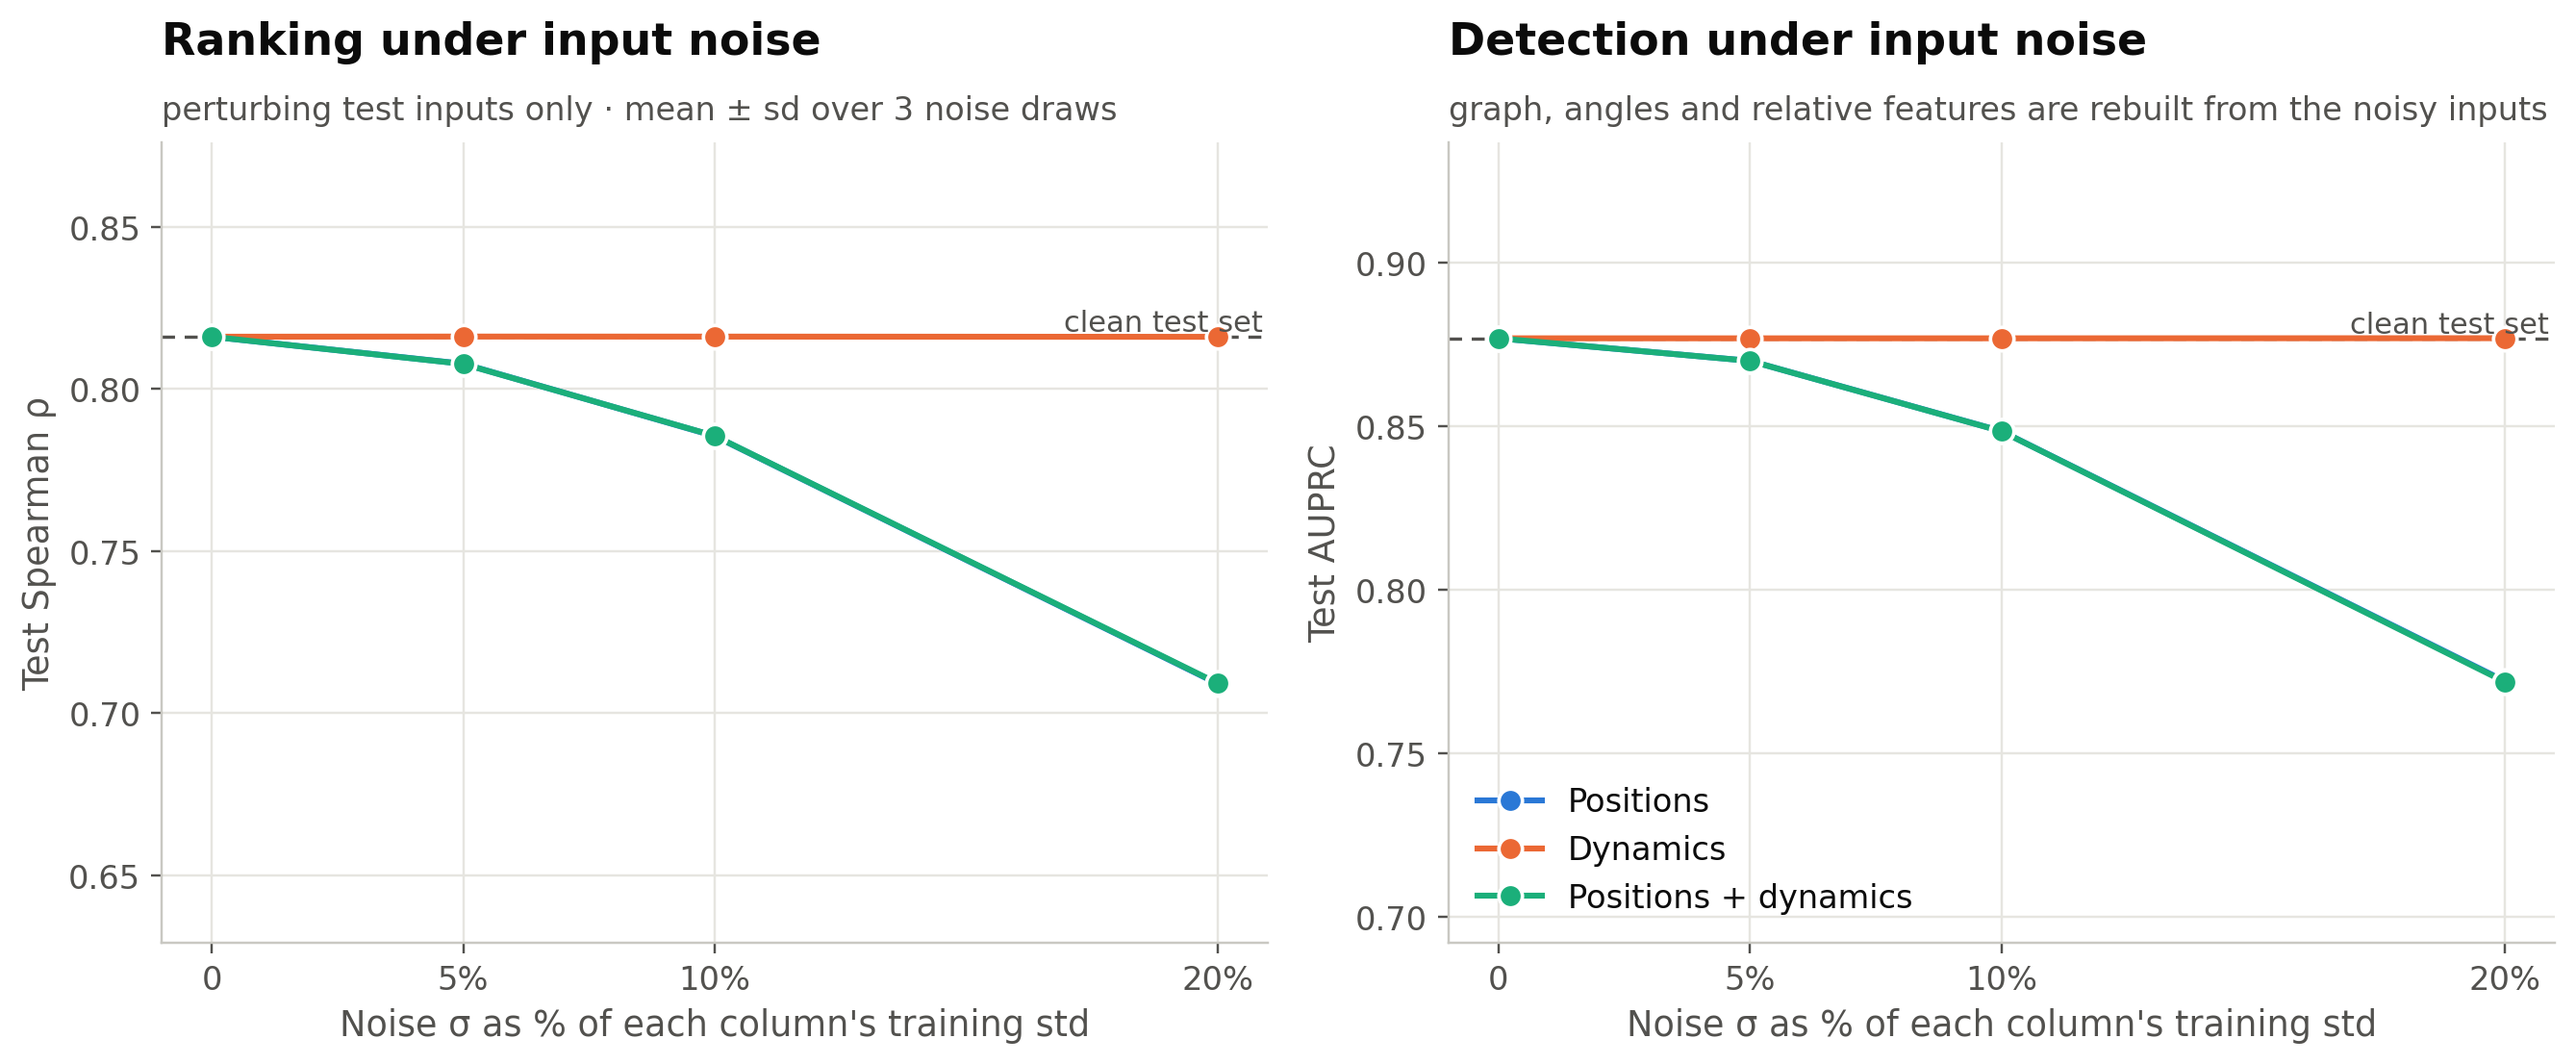
\includegraphics[width=0.85\textwidth]{robustness.png}
\caption{Test Spearman correlation and AUPRC when Gaussian noise is added to the test inputs; the proximity graph, angles and relative features are recomputed from the noisy values, and the curves for position noise and combined noise overlap. Velocity noise has no effect, whereas position noise lowers $\rho$ from 0.82 to 0.71 at 20\,\%, because it changes the graph and the neighbour-distance features the model relies on most.}\label{fig:rob}
\end{figure}

Adding noise to the velocities, speed, acceleration and angles barely changes the test metrics, even at
20\,\% of the training standard deviation (Figure~\ref{fig:rob}). Position noise has a much clearer effect.
The test $\rho$ falls from 0.816 to 0.808, 0.786 and 0.709 at 5, 10 and 20\,\% position noise, and AUPRC
falls from 0.877 to 0.771 by 20\,\%. Adding velocity noise on top of this does not make much difference.

One likely reason is that the edges are based on the 55-unit distance threshold. When the positions change,
some pairs gain or lose edges, and the neighbour distances and density features also change. The agent-level
model with temporal attention was less affected under the same 20\,\% position-noise setting, losing only
0.012 in $\rho$. Pooling information over a full mission can reduce the effect of independent noise at
individual timesteps, whereas the per-timestep model cannot use that information.

\subsection{Discussion and limitations}
\begin{itemize}
\item \textbf{Instantaneous and mission-level scores.} The per-timestep model can update its prediction as
a mission runs, and its output is usually stable over nearby steps. But it has lower accuracy early in the
mission and is more affected by position noise than the agent-level model. As a next step, I would try
averaging scores over a short recent window rather than over the entire mission.
\item \textbf{Training variation.} Most settings were trained using one random seed. The five runs of the
final configuration give some indication of variation, but repeating all ablations with multiple seeds
would make the comparisons more reliable.
\item \textbf{Simulator labels.} The criticality scores and labels come from the simulation. I have not
tested whether they predict the actual effect of removing an agent from a real swarm. In particular, the
node-removal validation proposed in Review~1 was not completed.
\item \textbf{Baseline comparison.} The Review~2 baselines were evaluated using a different split. Running
them again on the harder split would allow a fairer comparison with this model.

\end{itemize}

\section{Conclusions}
In this project, I trained a GINE-based model to rank agents and identify critical ones from a swarm graph at
each timestep. The main things I found are:
\begin{enumerate}[label=\arabic*.]
\item The model achieves test $\rho=0.816$ for per-timestep ranking and AUPRC 0.873 for classification,
compared with a random AUPRC of 0.39. Averaging the predicted scores over the mission gives $\rho=0.863$
and AUPRC 0.933 at the agent level.
\item It can handle the larger unseen swarm sizes (52--75 agents) and the held-out light and heavy
attrition conditions reasonably well. Small swarms and sparse obstacle fields are more difficult.
\item The predictions improve substantially as a mission progresses: ranking correlation increases
from about 0.59 at the beginning to 0.92 near the end. The predicted rankings are also very consistent
between nearby timesteps.
\item Adding a classification term to the ranking loss improves AUPRC by about 0.08 without reducing
test ranking quality. The best detection result is at latent size $d=12$, while the relative features
have little measurable effect at that size.
\item The network gives the most weight to local density and nearby-agent distances. Its main weakness
is position noise, which can change the graph itself; 20\,\% noise lowers test $\rho$ from about
0.82 to 0.71.
\end{enumerate}

Overall, the results suggest that graph-based prediction is promising for this simulated setting,
particularly when a ranking is needed during a mission. More training runs, controlled baseline
comparisons and tests on more realistic swarm behaviour are still needed before drawing stronger conclusions.

\begin{thebibliography}{9}\small
\bibitem{lalou2018cndp} M.~Lalou, M.~A.~Tahraoui, H.~Kheddouci, ``The critical node detection problem in networks: A survey,'' \emph{Computer Science Review}, 28:92--117, 2018.
\bibitem{teng2024drones} M.~Teng, C.~Gao, Z.~Wang, X.~Li, ``A communication-based identification of critical drones in malicious drone swarm networks,'' \emph{Complex \& Intelligent Systems}, 10(3):3197--3211, 2024.
\bibitem{fan2019drbc} C.~Fan, L.~Zeng, Y.~Ding, M.~Chen, Y.~Sun, Z.~Liu, ``Learning to identify high betweenness centrality nodes from scratch: A novel graph neural network approach,'' in \emph{Proc.\ CIKM}, pp.~559--568, 2019.
\bibitem{xu2019gin} K.~Xu, W.~Hu, J.~Leskovec, S.~Jegelka, ``How powerful are graph neural networks?'' in \emph{Proc.\ ICLR}, 2019.
\bibitem{hu2020gine} W.~Hu, B.~Liu, J.~Gomes, M.~Zitnik, P.~Liang, V.~Pande, J.~Leskovec, ``Strategies for pre-training graph neural networks,'' in \emph{Proc.\ ICLR}, 2020.
\bibitem{qin2010} T.~Qin, T.-Y.~Liu, H.~Li, ``A general approximation framework for direct optimization of information retrieval measures,'' \emph{Information Retrieval}, 13(4):375--397, 2010.
\end{thebibliography}


\clearpage
\appendix
\section{Design choices at $d=16$}\label{app:d16}
I repeated E2 and E3 with $d=16$ to check whether the results in Section~\ref{sec:design} change with
the latent size. Table~\ref{tab:d16} also shows the corresponding tests for the agent-level model
presented at the final review. That model uses additive attention to combine each agent's states
over time and produces one mission-level score per agent.

\begin{table}[!htbp]\centering\small
\caption{Ablations at $d=16$ on the test split. Per-timestep metrics are computed per agent-timestep; agent-level metrics per agent.}\label{tab:d16}
\begin{tabular}{@{}lllcccc@{}}\toprule
Model & Experiment & Variant & Train $\rho$ & Test $\rho$ & Test AUPRC & Test F1\\\midrule
Per-timestep & E2 & with relative features & 0.835 & 0.815 & 0.870 & 0.774\\
 & & without & 0.837 & 0.810 & 0.868 & 0.770\\
 & E3 & $\lambda=0.5$ & 0.836 & 0.810 & \textbf{0.874} & ---\\
 & & $\lambda=0$ & 0.851 & 0.815 & 0.774 & ---\\\midrule
Agent-level & E2 & with relative features & 0.938 & \textbf{0.835} & \textbf{0.948} & \textbf{0.881}\\
 & & without & 0.924 & 0.813 & 0.932 & 0.857\\
 & E3 & $\lambda=0.5$ & 0.924 & \textbf{0.852} & \textbf{0.936} & ---\\
 & & $\lambda=0$ & 0.924 & 0.820 & 0.805 & ---\\\bottomrule
\end{tabular}
\end{table}

\noindent The $d=16$ results tell a similar story for the per-timestep model: adding the relative
features gives only a small change, while including the classification loss increases AUPRC by
about 0.10 without a clear improvement in test ranking. For the agent-level model, both changes
help ranking more noticeably, by 0.022 and 0.032 in test $\rho$.

\begin{figure}[!htbp]\centering
\begin{subfigure}{0.49\textwidth}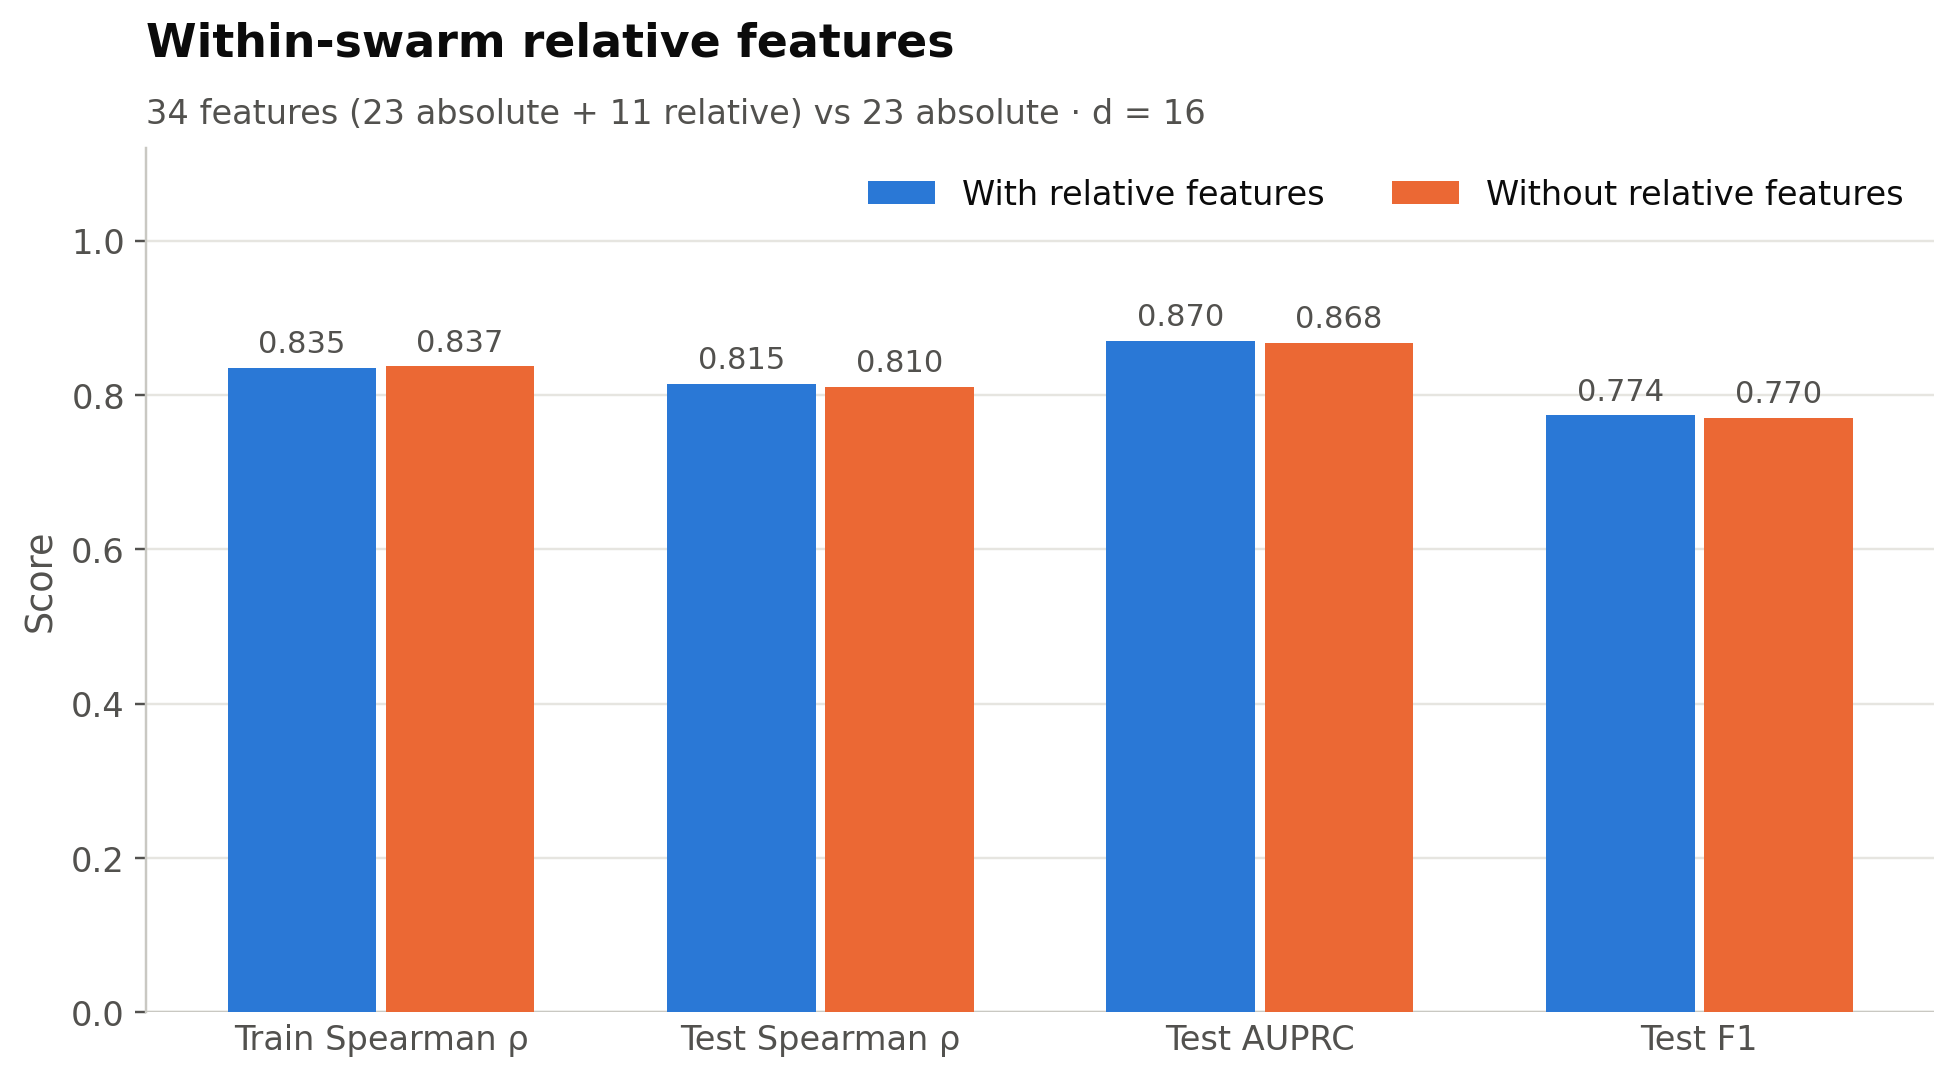
\includegraphics[width=\linewidth]{relative_vs_absolute_metrics_pt_d16.png}\caption{E2: with and without relative features.}\end{subfigure}\hfill
\begin{subfigure}{0.49\textwidth}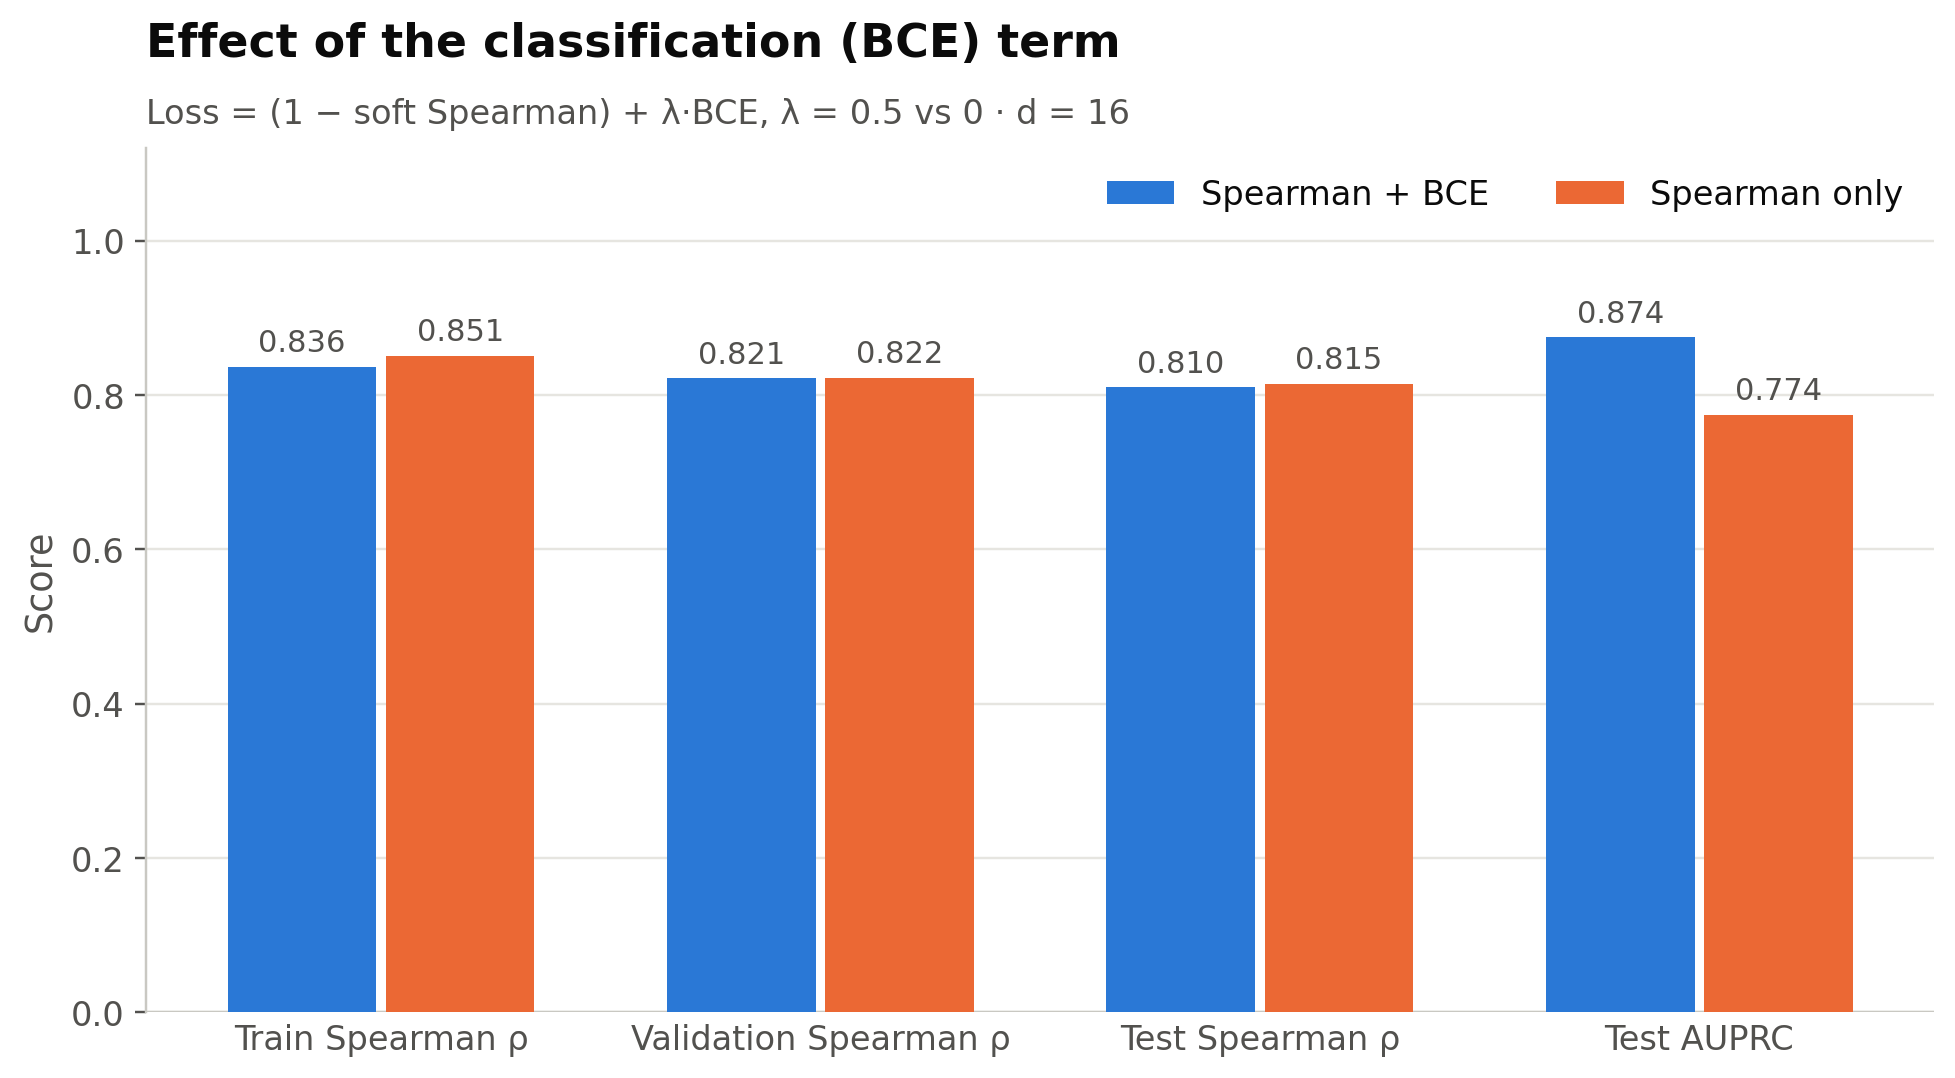
\includegraphics[width=\linewidth]{bce_ablation_metrics_pt_d16.png}\caption{E3: with and without the classification term.}\end{subfigure}
\caption{Design-choice experiments of the per-timestep model repeated with latent dimension $d=16$. As at $d=12$, the relative features have no measurable effect, and the classification term raises AUPRC by 0.10 without changing the test ranking.}\label{fig:d16}
\end{figure}

\clearpage
\section{Additional figures of the per-timestep model ($d=12$)}
\begin{figure}[!htbp]\centering
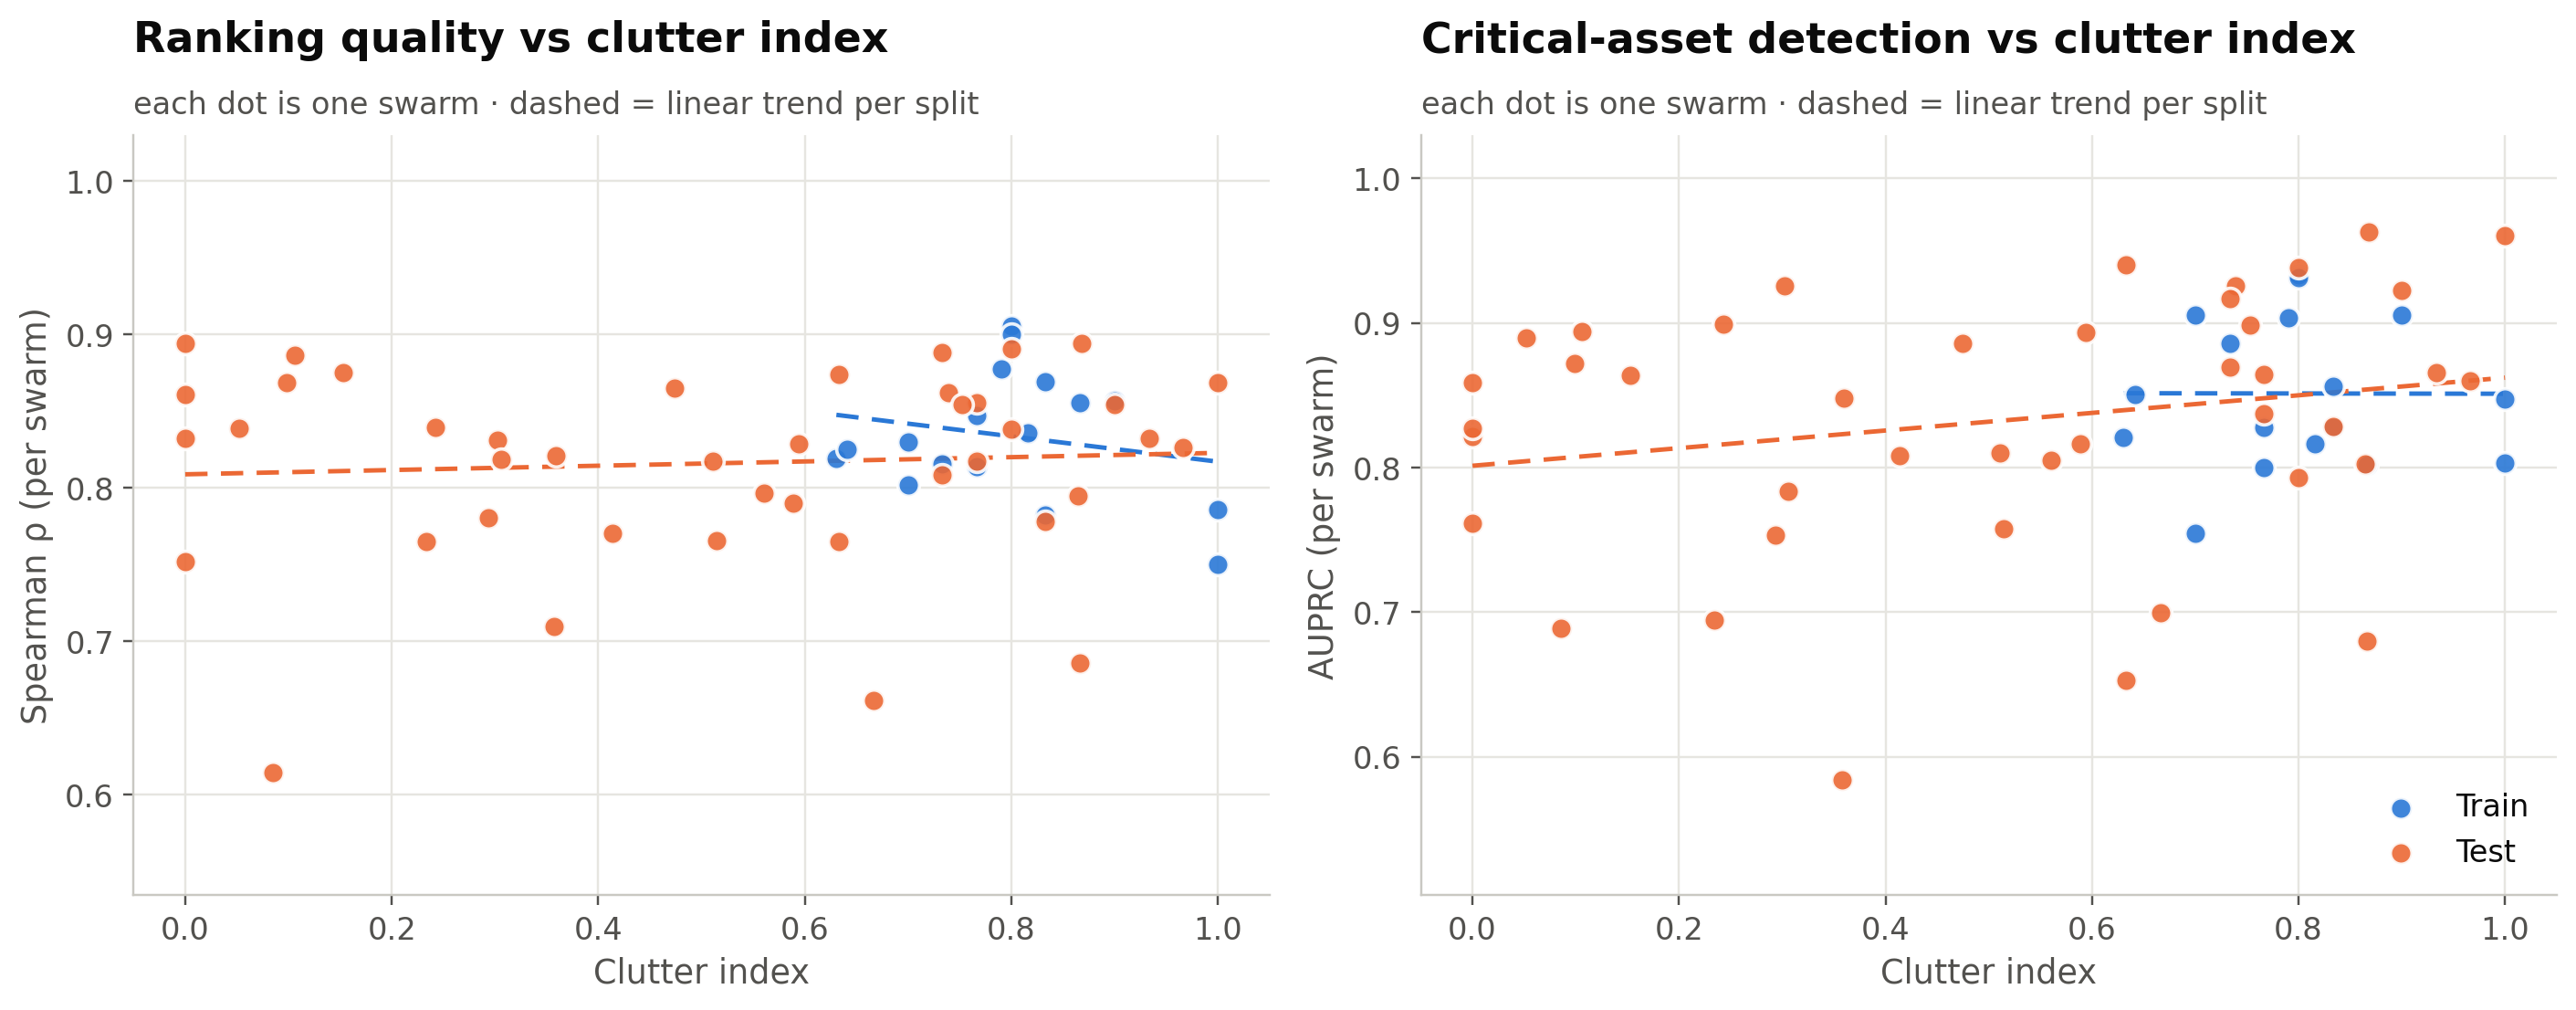
\includegraphics[width=0.85\textwidth]{performance_vs_clutter_index.png}
\caption{Per-swarm Spearman correlation and AUPRC against the clutter index, with linear fits for the training and test swarms. Neither
metric shows a clear trend with clutter.}\label{fig:obst}
\end{figure}

\begin{figure}[!htbp]\centering
\begin{subfigure}{0.49\textwidth}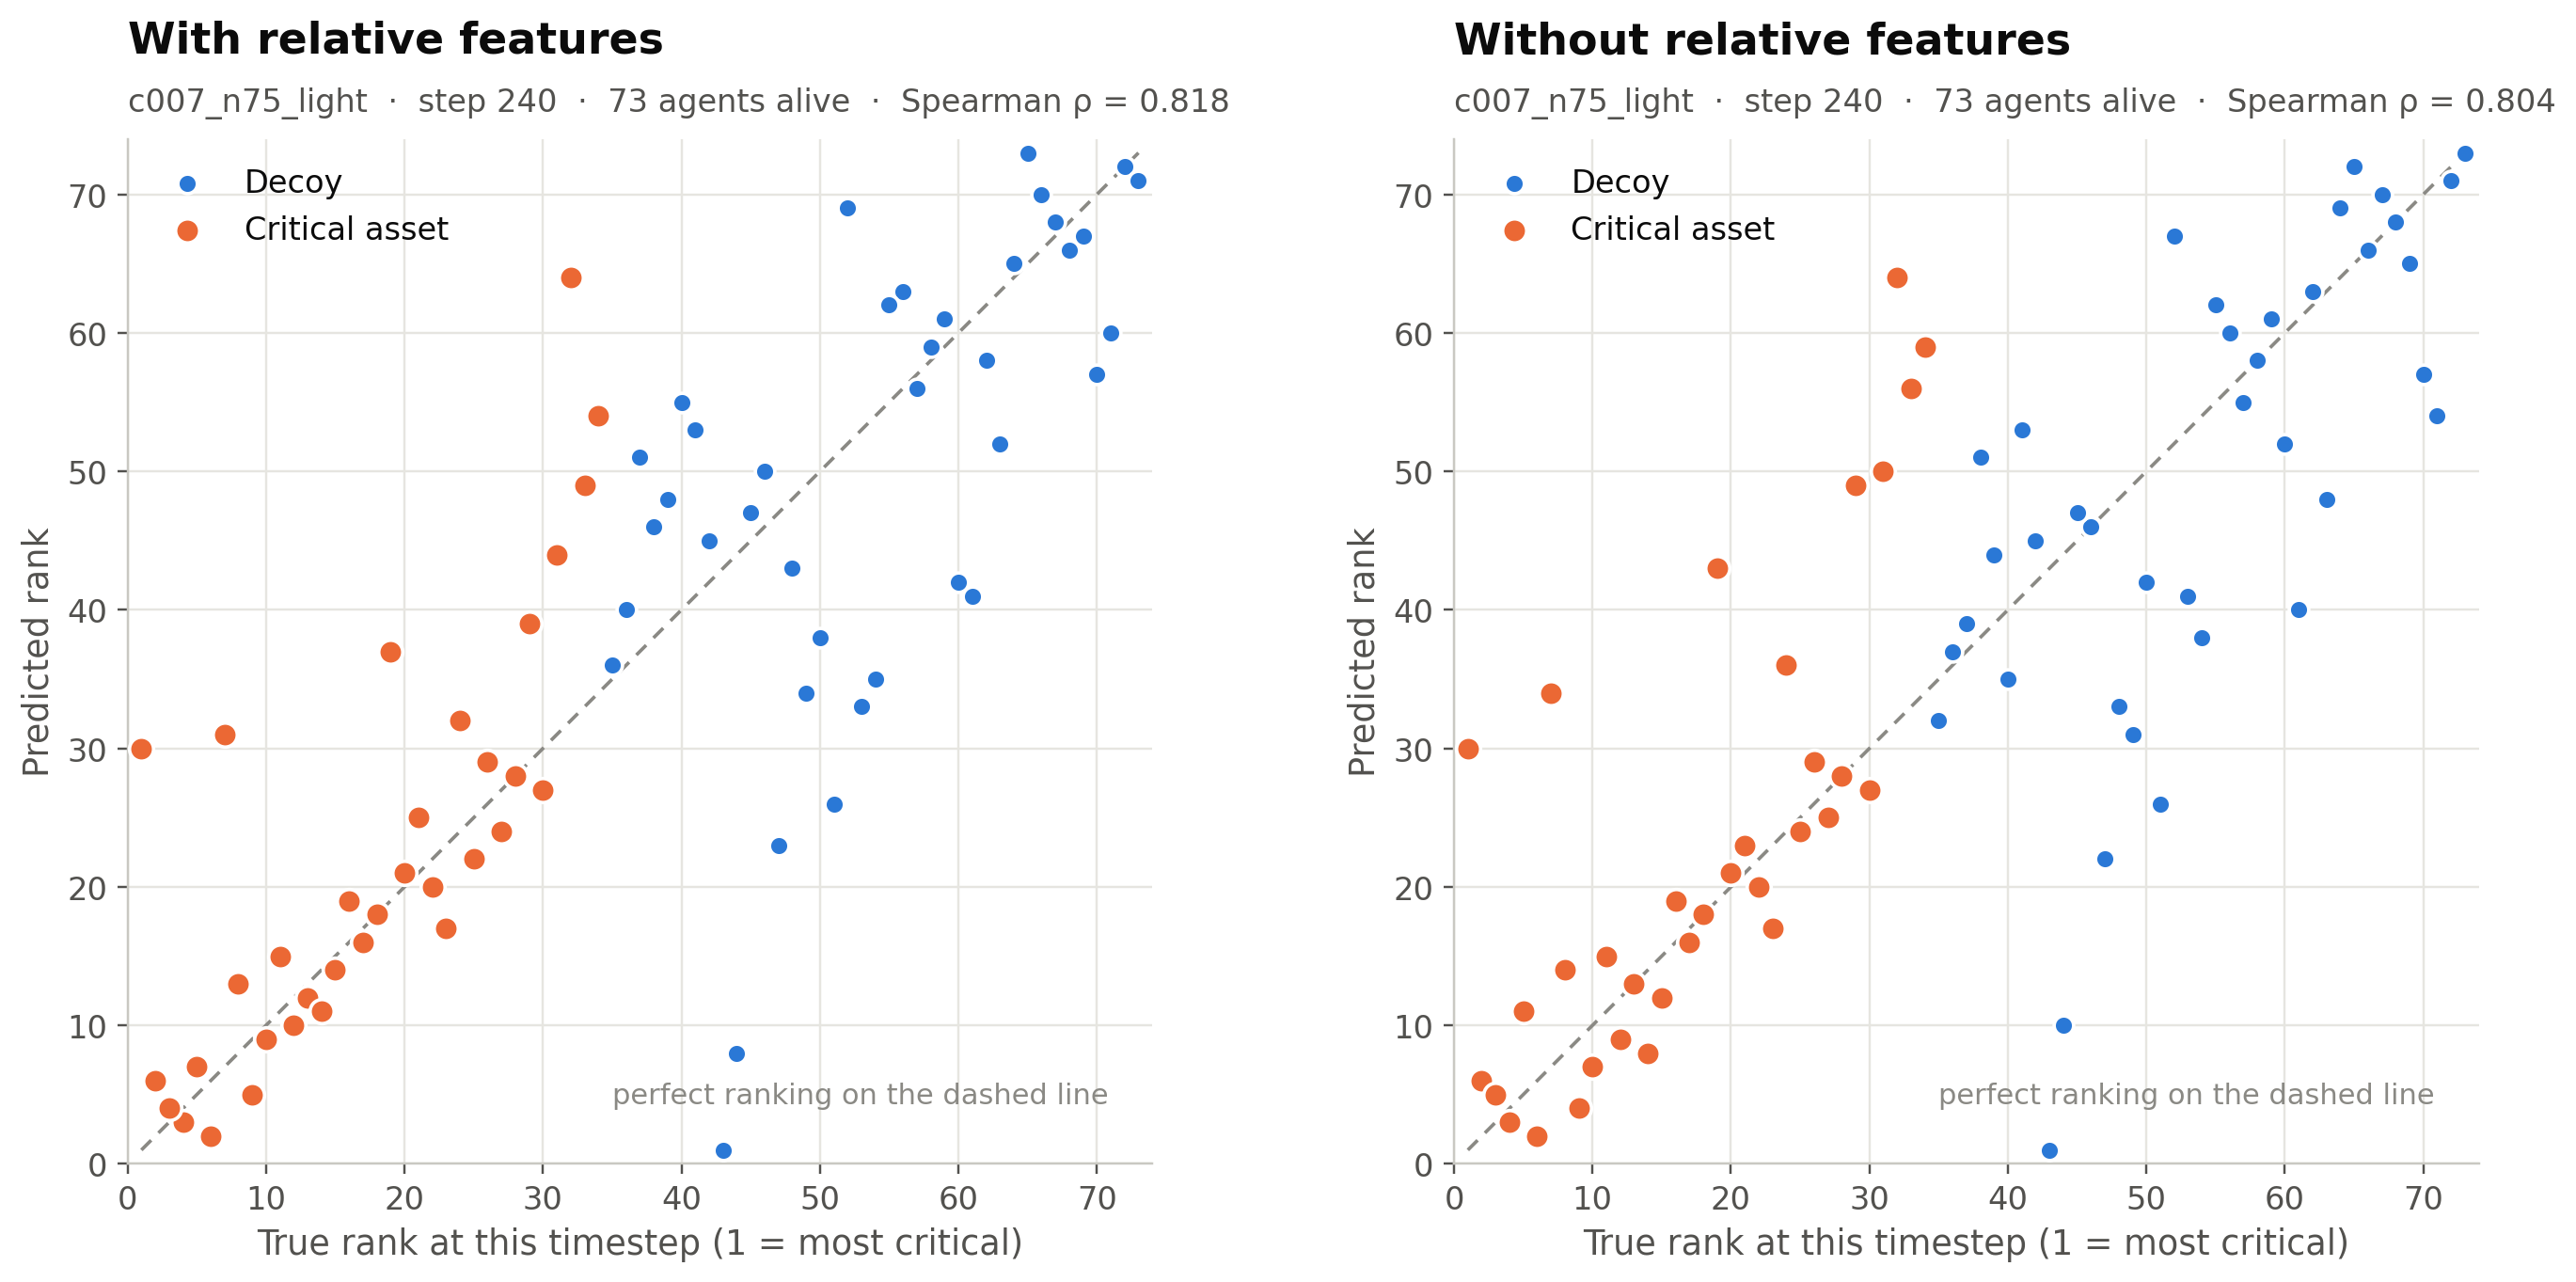
\includegraphics[width=\linewidth]{rank_agreement_relative_d12.png}\caption{E2: with and without relative features.}\end{subfigure}\hfill
\begin{subfigure}{0.49\textwidth}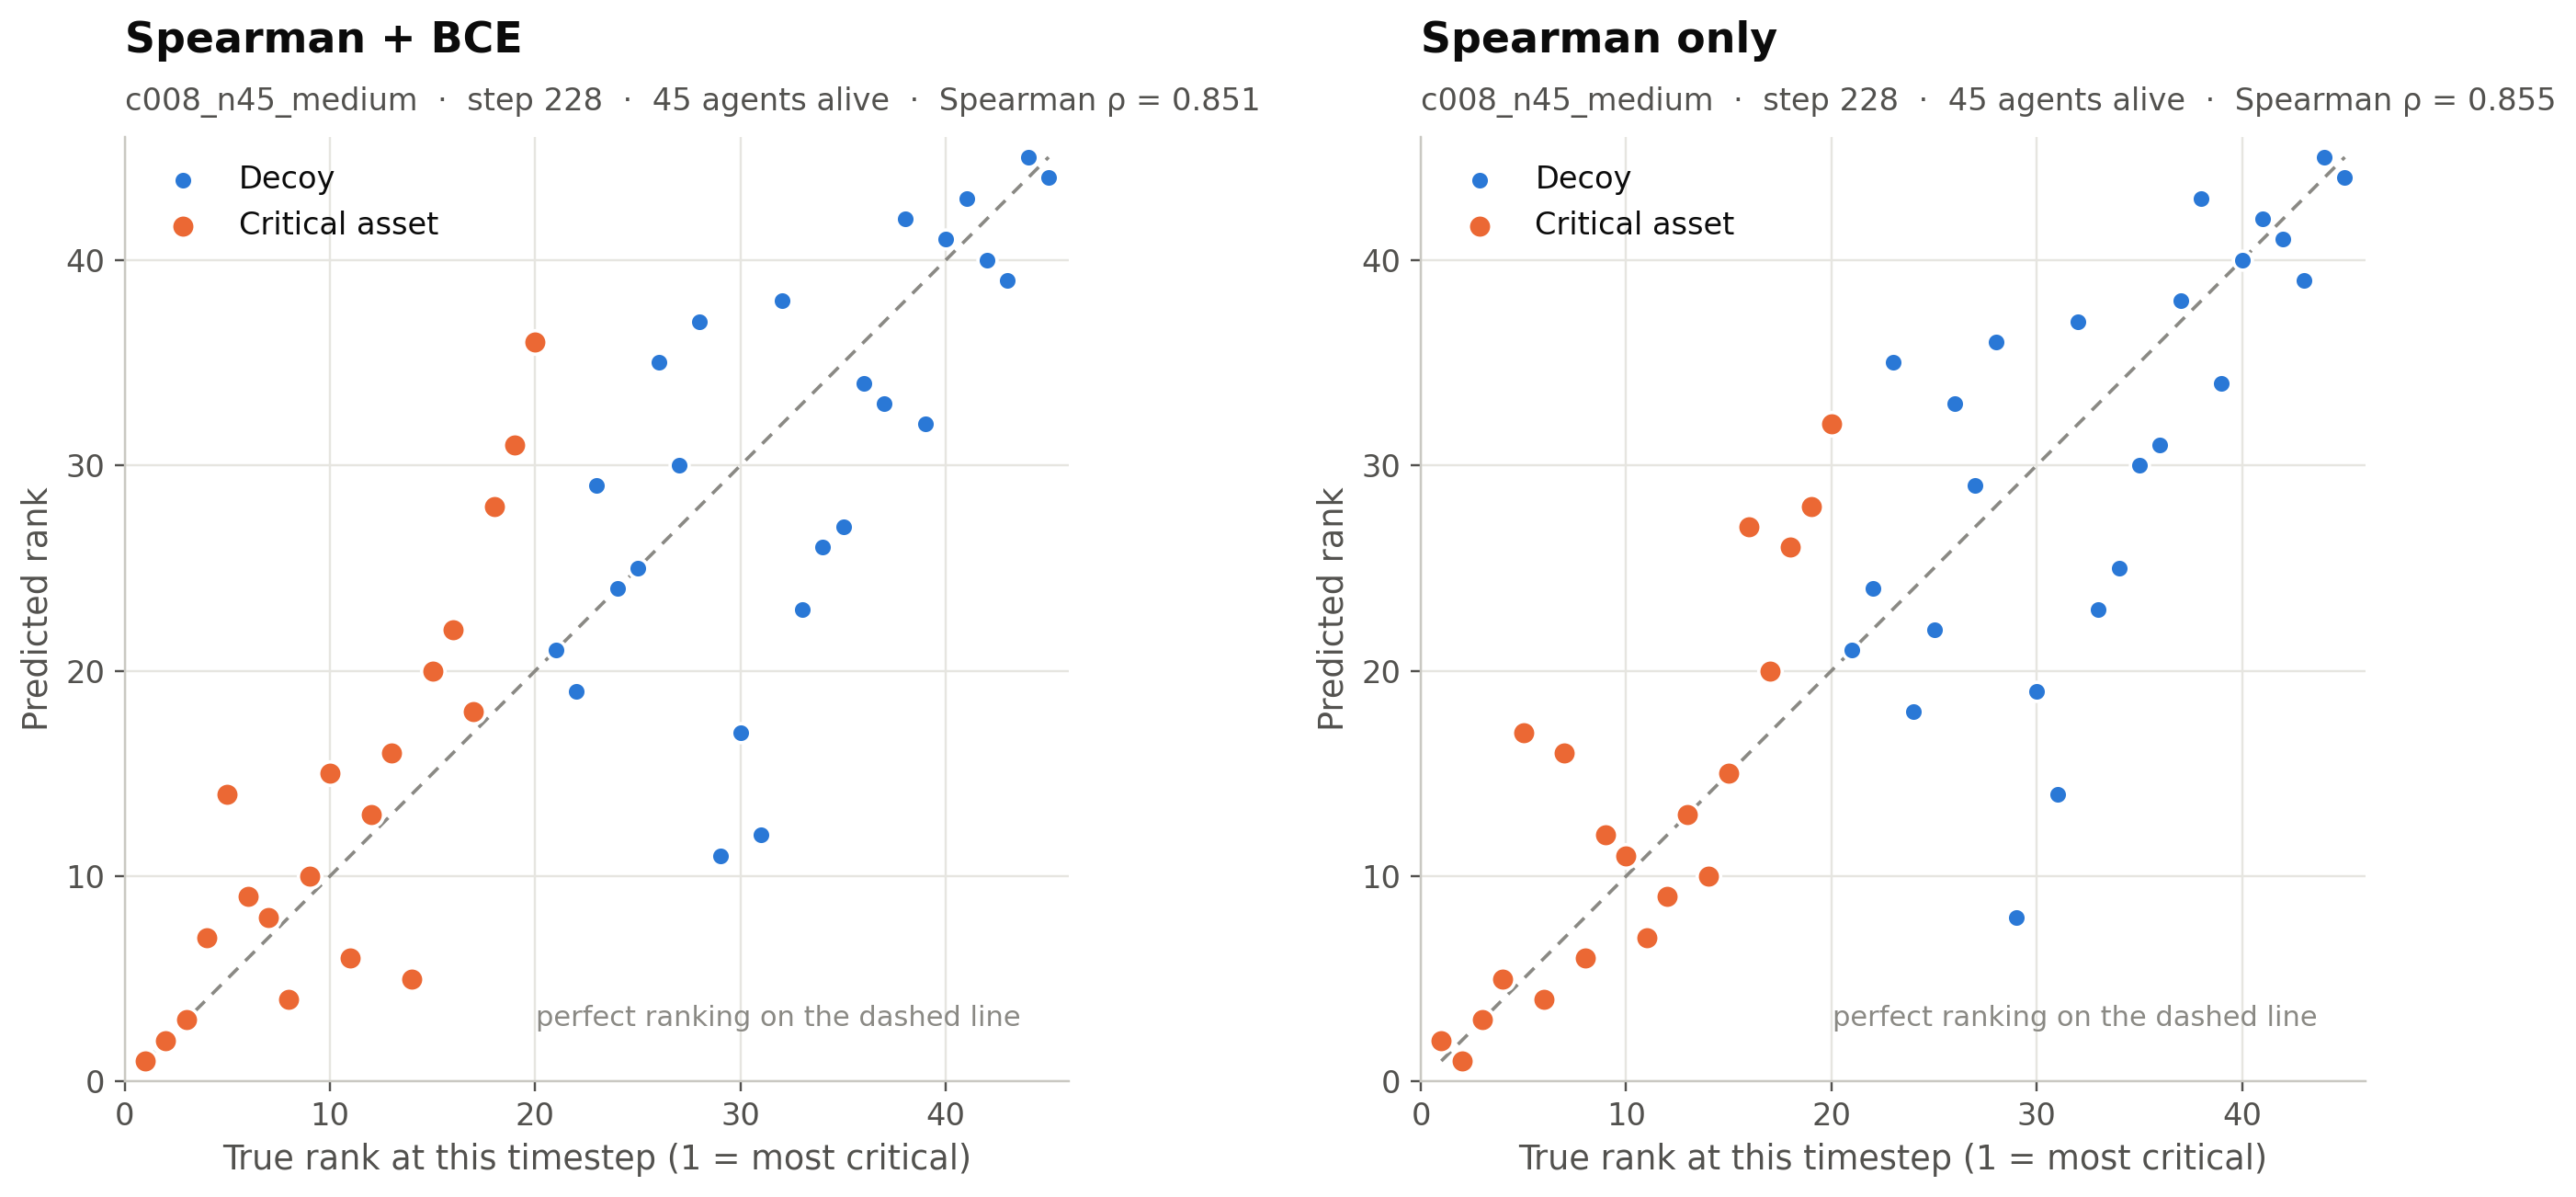
\includegraphics[width=\linewidth]{rank_agreement_bce_d12.png}\caption{E3: with and without the classification term.}\end{subfigure}
\caption{True and predicted ranks at one test timestep for the variants of E2 and E3 ($d=12$). In both cases the two variants rank the
agents almost identically ($\rho$ within 0.015), in line with the small differences in Table~\ref{tab:design}.}\label{fig:extra}
\end{figure}


\section{Evaluation metrics}\label{app:metrics}
\paragraph{Notation.} For a swarm $c$ and a sampled timestep $t$, $A(t)$ is the set of $n_t=|A(t)|$ alive agents, $s_i(t)$ the true
criticality score, $\hat s_i(t)$ the predicted score, $y_i(t)\in\{0,1\}$ the \texttt{is\_critical} label, and $r_i(t)$, $\hat r_i(t)$ the
ranks of $s_i(t)$ and $\hat s_i(t)$ among $A(t)$ (rank 1 = most critical; tied values receive their average rank).

\subsection*{Ranking metrics (computed at every timestep)}
\paragraph{Spearman's rank correlation} is the Pearson correlation of the two rank vectors,
\begin{equation}
\rho_t=\frac{\sum_{i\in A(t)}(r_i-\bar r)(\hat r_i-\bar{\hat r})}{\sqrt{\sum_{i}(r_i-\bar r)^2}\sqrt{\sum_{i}(\hat r_i-\bar{\hat r})^2}},
\qquad \rho_t=1-\frac{6\sum_i(r_i-\hat r_i)^2}{n_t(n_t^2-1)}\ \text{ without ties}.
\end{equation}
\paragraph{Kendall's $\tau_b$} counts concordant ($P$) and discordant ($Q$) agent pairs, i.e.\ pairs ordered the same or the opposite way by
$s$ and $\hat s$, with $T_s$ and $T_{\hat s}$ the pairs tied only in $s$ or only in $\hat s$:
\begin{equation}
\tau_b=\frac{P-Q}{\sqrt{(P+Q+T_s)(P+Q+T_{\hat s})}}.
\end{equation}
\paragraph{Precision@$k$} is the share of the true top-$k$ agents that are also in the predicted top-$k$,
\begin{equation}
\mathrm{P@}k=\frac{|\mathrm{Top}_k(s)\cap\mathrm{Top}_k(\hat s)|}{k},\qquad k\in\{1,5,10\}.
\end{equation}
\paragraph{NDCG@$k$} rewards placing highly critical agents near the top of the predicted list. With $\pi(m)$ the agent at predicted
position $m$ and the true score as the gain,
\begin{equation}
\mathrm{DCG@}k=\sum_{m=1}^{k}\frac{s_{\pi(m)}}{\log_2(m+1)},\qquad \mathrm{NDCG@}k=\frac{\mathrm{DCG@}k}{\mathrm{IDCG@}k},
\end{equation}
where IDCG@$k$ is the DCG of the ideal ordering by true score, so that $\mathrm{NDCG@}k\in[0,1]$.

\paragraph{Aggregation.} Each ranking metric $M_t$ is computed only at steps with at least two alive agents and non-constant true scores
($T_c$), averaged over the steps of the swarm, and then over the $C$ swarms of a split:
\begin{equation}
M_c=\frac{1}{|T_c|}\sum_{t\in T_c}M_t,\qquad \bar M=\frac{1}{C}\sum_{c=1}^{C}M_c,\qquad
\mathrm{sd}=\sqrt{\frac{1}{C-1}\sum_{c}(M_c-\bar M)^2}.
\end{equation}

\subsection*{Classification metrics (pooled over all agent-timesteps of a split)}
With the predicted label $\hat y_i(t)=\mathbf{1}[\hat s_i(t)\ge\theta]$ and the counts of true positives (TP), false positives (FP), false
negatives (FN) and true negatives (TN),
\begin{equation}
\begin{gathered}
\mathrm{Accuracy}=\frac{TP+TN}{TP+FP+FN+TN},\qquad
\mathrm{Precision}=\frac{TP}{TP+FP},\qquad
\mathrm{Recall}=\frac{TP}{TP+FN},\\[4pt]
F_1=\frac{2\,\mathrm{Precision}\cdot\mathrm{Recall}}{\mathrm{Precision}+\mathrm{Recall}}.
\end{gathered}
\end{equation}
\paragraph{Threshold.} $\theta$ is chosen on the validation split and then kept fixed for the test split,
\begin{equation}
\theta^\ast=\arg\max_{\theta\in\{0.01,\,0.02,\,\ldots,\,0.99\}}F_1^{\mathrm{val}}(\theta).
\end{equation}
\paragraph{AUPRC (average precision).} Sorting all predictions by decreasing score and taking the precision $P_n$ and recall $R_n$ at the
$n$-th threshold,
\begin{equation}
\mathrm{AUPRC}=\sum_{n}(R_n-R_{n-1})\,P_n .
\end{equation}
A random scorer has AUPRC equal to the share of positives, $\pi=N_{\mathrm{pos}}/N$ (0.39 here), which is the chance level quoted in the text.
\paragraph{ROC-AUC} is the probability that a randomly chosen critical agent-timestep receives a higher score than a randomly chosen
non-critical one,
\begin{equation}
\mathrm{ROC\text{-}AUC}=\frac{1}{N_{\mathrm{pos}}N_{\mathrm{neg}}}\sum_{a:\,y_a=1}\ \sum_{b:\,y_b=0}\Big(\mathbf{1}[\hat s_a>\hat s_b]+\tfrac12\,\mathbf{1}[\hat s_a=\hat s_b]\Big);
\end{equation}
its chance level is 0.5.

\subsection*{Agent-level and temporal metrics}
\paragraph{Scores averaged over the mission.} For agent $i$ alive at the steps $T_i$, the per-timestep predictions are averaged,
$\bar s_i=\frac{1}{|T_i|}\sum_{t\in T_i}\hat s_i(t)$, and compared with the mission-level targets $\frac{1}{|T_i|}\sum_{t\in T_i}s_i(t)$
(Spearman per swarm, averaged over swarms) and $\max_{t\in T_i}y_i(t)$ (pooled AUPRC).
\paragraph{Ranking consistency.} For consecutive sampled steps $t$ and $t'$, the Spearman correlation between $\hat s(t)$ and
$\hat s(t')$ over the agents alive at both steps; the same quantity for the true scores gives the reference value.
\paragraph{Per-swarm AUPRC.} AUPRC computed over the agent-timesteps of one swarm, used for the condition plots and averaged over swarms
where reported.


\section*{Use of AI}
\addcontentsline{toc}{section}{Use of AI}
Claude (Anthropic) was used to help plot the figures, and ChatGPT (OpenAI) was used to help revise the wording and readability of this report. No new experimental results were generated during the writing revision.

\end{document}
